%% Manuscript for Chaos: An Interdisciplinary Journal of Nonlinear Science (AIP Publishing), REVTeX 4.2.
%% Sources: sections/*.tex; figures/*.pdf (make_figures.py); refs.bib (build.py, from data/bibliography.json).
%% Build: python paper2_esn/chaos/build.py  ->  manuscript.tex (one flattened file) and manuscript.pdf
\documentclass[aip,cha,reprint,amsmath,amssymb,longbibliography]{revtex4-2}

\usepackage{graphicx}
\usepackage{amsthm}
\usepackage{bm}
\usepackage{xcolor}
\usepackage[colorlinks=true,linkcolor=blue!55!black,citecolor=blue!55!black,urlcolor=blue!55!black]{hyperref}

% float placement: fill pages with figures instead of deferring them past the references
\renewcommand{\topfraction}{0.95}
\renewcommand{\bottomfraction}{0.8}
\renewcommand{\textfraction}{0.05}
\renewcommand{\floatpagefraction}{0.75}
\renewcommand{\dbltopfraction}{0.95}
\renewcommand{\dblfloatpagefraction}{0.75}
\setcounter{topnumber}{3}
\setcounter{bottomnumber}{2}
\setcounter{totalnumber}{5}
\setcounter{dbltopnumber}{3}

\newtheorem{theorem}{Theorem}
\newtheorem{lemma}{Lemma}
\newtheorem{proposition}{Proposition}
\newtheorem{corollary}{Corollary}
\theoremstyle{definition}
\newtheorem{definition}{Definition}
\newtheorem{remark}{Remark}
\newcommand{\ind}{\operatorname{ind}}
\newcommand{\Uin}{U_{\mathrm{in}}}
% text the author must supply before submission (printed in red)
\newcommand{\placeholder}[1]{\textcolor{red}{[#1]}}
% a number still to be filled from paper2_esn/chaos/numbers (printed in red until replaced)
\newcommand{\num}[1]{\textcolor{red}{#1}}

\begin{document}

\title[Do trained models keep attractors hidden?]{Do trained models keep attractors hidden? Forced spurious equilibria and a survival law for hiddenness}

\author{Maksim Elisov}
\email{maksimelisov2003@gmail.com}
\affiliation{Samara National Research University, Moskovskoye Shosse 34, Samara 443086, Russia}

\date{\today}

\begin{abstract}
An attractor is hidden if its basin avoids small neighborhoods of all equilibria, so it cannot be found from the
equilibria. We ask whether a trained model that reproduces a hidden attractor keeps it hidden from its own
equilibria; mostly it does not. Across 3710 hidden attractors reproduced by models of four classes trained on
six regimes, the share still hidden falls from 0.99 for perceptrons without unstable equilibria in the region of the true
system to about one third with one and to 0.03 or less with nine or more; model class, reservoir size and depth act mainly
through this number. Degree theory fixes the bookkeeping: a bounded model with nondegenerate equilibria has an odd
number of them, and every extra pair contains an unstable one. If the
index sum $s$ of the true equilibria is not one, as for Chua's circuit ($s=-1$), a bounded model must miss a true
equilibrium or add spurious ones; with no true equilibria ($s=0$) it always has one, and the reproduced attractor is
self-excited in all 29 cases. An equilibrium excites an attractor exactly when its local unstable manifold reaches the
closure of the basin. Transients toward the visible attractor raise survival, and a training penalty on unstable
equilibria raises it in two-layer perceptrons from 0.27 to 0.994 at unchanged median one-step error. Survival is not
fidelity: few hidden reproductions also have the visible equilibrium and a correct basin. Generic models do not infer
hidden attractors the data do not touch.
\end{abstract}

\maketitle

\begin{quotation}
Some attractors of nonlinear systems are hidden: no trajectory started near an equilibrium leads to them, so the usual
analysis, which starts at the equilibria, misses them. Neural networks trained on time series are now widely used in place
of equations, and they can reproduce such an attractor. This paper asks whether the attractor also stays hidden inside the
model. Often it does not. A trained model has equilibria of its own, often more than the true system, and in some systems
topology forces extra ones on any model with bounded output that copies the true equilibria. An attractor becomes
reachable from an equilibrium as soon as one of the unstable directions of that equilibrium leads into its basin. Across
ten thousand models of four kinds, the chance that the attractor stays hidden is set mainly by a single number, the count
of unstable equilibria in the region where the system lives. Generic models also do not discover hidden attractors that their data never
approach.
\end{quotation}

\section{Introduction}
\label{sec:intro}

An attractor is hidden if its basin does not intersect small neighborhoods of the equilibria, so that it cannot be found
by starting trajectories near an equilibrium; otherwise it is self-excited.\cite{LeonovKuznetsov2013,Dudkowski2016} Hidden
attractors were first located in Chua's circuit\cite{Leonov2011PLA} and are now known in systems without equilibria, with
lines of equilibria and with a single stable equilibrium.\cite{Dudkowski2016,Molaie2013,JafariSprott2013,WangChen2012} The
distinction matters in practice because the standard analysis of a system starts at its equilibria: their stability and
the unstable manifolds of the saddles reveal the self-excited regimes, while a hidden regime stays invisible. In control
systems, phase-locked loops and drilling rigs, such regimes coexist with a stable operating point and appear only after a
large perturbation.\cite{Kuznetsov2020JCSSI}

Models trained from data increasingly stand in for equations. Reservoir computers running in closed loop reproduce chaotic
attractors and their Lyapunov spectra\cite{JaegerHaas2004,Pathak2017Chaos,LuHuntOtt2018} and forecast large spatiotemporal
systems;\cite{Pathak2018PRL} next-generation reservoir computers,\cite{Gauthier2021NGRC} recurrent networks trained by
backpropagation,\cite{Vlachas2020Backprop} sparse regression\cite{Brunton2016SINDy} and neural ordinary differential
equations\cite{Chen2018NeuralODE} serve the same purpose. Beyond forecasting, such models are asked for global information:
the coexisting attractors of a multistable system and their basins,\cite{Roy2022Multistability,Liu2025HiddenDynamics} and
even attractors absent from the training data. A reservoir trained on one attractor of the Li--Sprott system, which has no
equilibria, reproduces its unseen coexisting attractors,\cite{Rohm2021,Rohm2022Unseen} and a reservoir trained on the
trajectories of one basin reproduces other basins and chaotic attractors.\cite{Norton2025Unseen}

A trained model is, however, a dynamical system of its own, often of dimension in the hundreds, and its behavior away from
the data is not controlled by training. Reservoirs acquire mirror attractors from the symmetry of their
equations,\cite{HerteuxRath2020} extra saddles that organize their dynamics,\cite{Kabayama2025PseudoLorenz} untrained
attractors and fixed points,\cite{Flynn2021,Hart2024CLE,Norton2025Unseen} and spurious slow modes that pull trajectories to
fixed points;\cite{Oishi2026FastSlow} untrained attractors have been argued to be intrinsic to learning systems with a
bounded state space.\cite{OHagan2025Confabulation} Generalization across basins is impossible in general without prior
structure.\cite{Goring2024OOD} Most of this literature treats spurious behavior as a symptom of imperfect training, and it
studies attractors that are either visible in the data or have no equilibria nearby.

A hidden attractor of a system with equilibria is the hardest case of this kind. Reproducing it requires the model to get
right not only the attractor but also the neighborhoods of all equilibria, including equilibria that the true system does
not have. A model can reproduce the attractor faithfully and still place an unstable equilibrium whose neighborhood leads to
it; the attractor then becomes self-excited in the model, and the model gives the wrong answer for states near its
equilibria. Reservoir computers have been trained on systems with hidden attractors,\cite{Xu2024SelfESN,Mahata2025Extreme}
and one study predicted the basin of the stable equilibrium of the Wang--Chen system next to what is, at its parameters, a
hidden cycle,\cite{Liu2025HiddenDynamics} but to our knowledge no work has checked whether a reproduced attractor stays
hidden with respect to the equilibria of the model; the closest works are those just cited and the index-theoretic
results for threshold-linear and Hopfield networks discussed in Sec.~\ref{sec:degree}.

This paper asks whether trained models keep hidden attractors hidden, and answers it for about $10^4$ models of four
classes trained on six regimes of four systems with hidden attractors, plus one weakly hidden control; the survival curves
rest on $3710$ reproductions of a hidden attractor, and a full-protocol ensemble of echo state networks adds $581$. The answer is mostly
no. Topology fixes the bookkeeping of a model's
equilibria and, in some systems, forces spurious ones on models that copy the true equilibria; training decides how many unstable equilibria the model has; and
their number in the region of the true system largely decides whether hiddenness survives. We make four contributions.
\begin{enumerate}
\item We adapt classical degree theory to trained models (Theorem~\ref{thm:degree}): a bounded model has an odd number of
equilibria, at least $(K-1)/2$ of them unstable, and an index sum different from $1$ certifies that a numerically found set
of equilibria is incomplete, a check we use throughout.
\item A bounded model that reproduces the true equilibria with their indices must have spurious equilibria of total index
$1-s$, where $s$ is the index sum of the true equilibria (Proposition~\ref{prop:forced}). For Chua's circuit in regime~I,
$s=-1$, and no bounded model in our ensembles reproduces all three equilibria; for the equilibrium-free system of R\"ohm
\textit{et al.},\cite{Rohm2021} $s=0$, every model has a spurious equilibrium, and the reproduced training attractor becomes
self-excited.
\item An attractor of the model is excited from an equilibrium exactly when the local unstable manifold of the equilibrium
reaches the closure of its basin (Proposition~\ref{prop:manifold}), which reduces the excitation test to the unstable
subspace.
\item The probability that a reproduced hidden attractor stays hidden falls with the number of unstable equilibria of the
model inside the region of the true system, similarly for echo state networks, one- and two-layer perceptrons and residual
networks; model class, reservoir size and depth act mainly through this number. Data from the basin of the visible
attractor raise survival. A penalty on unstable equilibria during training, which removes
them at fixed data, raises survival from $0.27$ to $0.994$ at an unchanged one-step error. Generic models do not reproduce a
hidden attractor that the data do not touch; a model whose function class contains the Euler step of the true vector
field sometimes does.
\end{enumerate}

Section~\ref{sec:setting} defines the models, the notion of hiddenness for a model and the test systems.
Section~\ref{sec:theory} states the theory, and Sec.~\ref{sec:methods} describes the ensembles and the labeling protocol.
Section~\ref{sec:results} tests the theory, measures the survival law and the effect of the data, and
Sec.~\ref{sec:discussion} discusses what this means for the use of trained models.

\section{Setting}
\label{sec:setting}

\subsection{Models as maps}
\label{sec:models}

All models considered here are autonomous maps that are iterated to produce a trajectory. An echo state
network\cite{Jaeger2001EchoState,LukoseviciusJaeger2009Reservoir} has the reservoir update
$r_{k+1}=\tanh(Wr_k+W_{\mathrm{in}}u_k+b)$ with a fixed random matrix $W$, input matrix $W_{\mathrm{in}}$ and bias $b$, and
a linear readout $u_k=W_{\mathrm{out}}r_k$ fitted by ridge regression. In closed loop the output is fed back as the input,
and the model is the map
\begin{equation}
F(r)=\tanh(Ar+b),\qquad A=W+W_{\mathrm{in}}W_{\mathrm{out}},
\label{eq:esn}
\end{equation}
on $\mathbb{R}^N$, with $N$ between $50$ and $2000$ for the trained networks. The other three classes act directly on the
normalized physical state
$u=(x-\bar x)/\sigma$, with the mean $\bar x$ and the standard deviation $\sigma$ of the training data taken per
coordinate: the one-hidden-layer perceptron (``mlp'') $F(u)=W_2\tanh(W_1u+b_1)+b_2$, the two-hidden-layer
perceptron (``mlp2'') $F(u)=W_3\tanh\bigl(W_2\tanh(W_1u+b_1)+b_2\bigr)+b_3$, and the residual network (``res'')
$F(u)=u+W_2\tanh(W_1u+b_1)+b_2$, a forward-Euler step of a neural vector
field.\cite{He2016ResNet,E2017Proposal,HaberRuthotto2018Stable} The first three classes have bounded output; the residual
network does not, and its trajectories can escape to infinity as those of the true systems do.

The equilibria of a model are the fixed points of its map. An equilibrium is unstable if $DF$ has an eigenvalue of
modulus greater than $1$. We write $U$ for the number of unstable equilibria found and $\Uin$ for the number of those whose
physical image ($W_{\mathrm{out}}r^*$ for the echo state network, $\sigma u^*+\bar x$ otherwise) lies in the region $Q$ of the
true system (Table~\ref{tab:systems}). For the perceptrons almost all unstable equilibria lie in $Q$, while residual networks
have on average one or two more outside it (Sec.~\ref{sec:classes}); for echo state networks we count all equilibria and
write $U$.

\subsection{Hidden attractors of a model}
\label{sec:hidden}

An attractor $\mathcal{A}$ of a map or flow, with basin $B$, is \emph{excited} from an equilibrium $e$ if $B$ intersects
every neighborhood of $e$. It is \emph{self-excited} if it is excited from at least one equilibrium and \emph{hidden}
otherwise.\cite{LeonovKuznetsov2013,Dudkowski2016} The definition is the same for maps, which have hidden attractors of
their own;\cite{Jiang2016Maps} a trained model is a map even when the true system is a flow. We consider attractors with an open basin (local attractors
in the sense of Leonov and Kuznetsov), which includes the chaotic attractors and limit cycles of the true systems; for them
an intersection of $B$ with a neighborhood of $e$ is open and has positive measure, which is what a numerical test can
detect. Attractors in Milnor's sense,\cite{Milnor1985Attractor} whose basin need not be open, would need a measure-theoretic
version of the definition. Hiddenness is a property of the pair
(attractor, set of equilibria), so the same attractor can be hidden in the true system and self-excited in a model that
has different equilibria.

A model \emph{reproduces} a hidden attractor of the true system if trajectories started from states on the true attractor
settle on a model attractor of the same type (chaotic or regular) that is close to it in two senses: the normalized
distance of first and absolute moments, $\Delta_{\mathrm{att}}$, and the Hausdorff distance relative to the attractor
diameter, $d_H$, are both below $0.2$ (Appendix~\ref{app:protocol}). The question of this paper is whether a reproduced
attractor stays hidden, now with respect to the equilibria of the model. We call the fraction of reproductions in which it
does the \emph{survival} probability.

\subsection{True systems}
\label{sec:systems}

\begin{table*}
\caption{Test systems. Equilibria are listed with their flow-map index $\iota$ in parentheses, Eq.~\eqref{eq:trueindex};
$s$ is the index sum. $p_B$ is the fraction of uniform initial conditions in the region $Q$ that reach the hidden
attractors (both of them for Chua's circuit); $\Delta t$ is the sampling interval of the training series. Equations and
regions are given in Appendix~\ref{app:systems}. $^{a}$Hidden only in a weak sense: not reached from the stable half-line of
equilibria, but reached from the segment $0.35\lesssim z\lesssim2.2$ of the unstable one, hence self-excited in the strict
sense; reported separately (Sec.~\ref{sec:systems}).}
\label{tab:systems}
\begin{ruledtabular}
\begin{tabular}{lllllllll}
Regime & System & Parameters & Equilibria ($\iota$) & $s$ & Hidden & Visible & $p_B$ & $\Delta t$ \\
\hline
SE3 & one stable equilibrium & -- & stable ($+$) & $1$ & chaotic & equilibrium & 0.152 & 0.2 \\
SE11 & one stable equilibrium & -- & stable ($+$) & $1$ & chaotic & equilibrium & 0.00827 & 0.15 \\
LE1 & line of equilibria & $a=15$, $b=1$ & line $x=y=0$ (stable for $z<0$) & -- & chaotic$^{a}$ & equilibria & 0.00127 & 0.16 \\
WC & Wang--Chen & $a=0.006$ & stable ($+$) & $1$ & chaotic & equilibrium & 0.67 & 0.18 \\
WC$'$ & Wang--Chen & $a=0.03$ & stable ($+$) & $1$ & cycle & equilibrium & 0.668 & 0.18 \\
Chua I & Chua's circuit & set I & 2$\times$ saddle-focus ($-$), stable ($+$) & $-1$ & 2$\times$ chaotic & equilibrium & 0.0369 & 0.07 \\
Chua II & Chua's circuit & set II & saddle-focus ($-$), 2$\times$ stable ($+$) & $1$ & 2$\times$ chaotic & cycle & 0.00274 & 0.05 \\
\end{tabular}
\end{ruledtabular}
\end{table*}


Seven regimes of five three-dimensional flows with attractors reported as hidden and at least one equilibrium make up the
test set (Table~\ref{tab:systems}); six of them are hidden in the strict sense.\cite{Molaie2013,JafariSprott2013,WangChen2012,Leonov2011PLA,Stankevich2017} Two systems from
the family with one stable equilibrium (SE3 and SE11) have a hidden chaotic attractor next to a stable focus. LE1 has a line
of equilibria $x=y=0$, stable for $z<0$ and unstable for $z>0$. Its attractor is hidden only in the weaker sense of
Jafari and Sprott,\cite{JafariSprott2013} who noted that its basin meets the line in some portions: it is not reached from
the stable half-line, but it is reached from a segment of the unstable one, $0.35\lesssim z\lesssim2.2$: trajectories
started at distance $10^{-8}$ from the line reach it along $43\%$ of the directions on average for $0.3<z\le1$, and along
all of them at some points (Appendix~\ref{app:systems}).
In the sense of Sec.~\ref{sec:hidden} the attractor of LE1 is therefore self-excited. We report LE1 separately, as a
control in which the true system itself has exciting equilibria: for it, an attractor that is not excited in a model
marks a loss of faithfulness rather than the survival of hiddenness. All pooled statistics use the other six regimes.
The Wang--Chen system has a single stable equilibrium and a hidden chaotic attractor at
$a=0.006$ that becomes a hidden limit cycle at $a=0.03$; its basin covers about two thirds of the region. Chua's circuit is
taken in the two classical regimes: in regime~I a stable origin and two saddle-foci coexist with two symmetric hidden
chaotic attractors; in regime~II two stable equilibria and an unstable origin coexist with a large visible limit cycle
and two hidden chaotic attractors. The equilibria of LE1 are not isolated and have no index, so
Proposition~\ref{prop:forced} applies to the other six regimes; of these, only Chua~I has $s\neq1$. As a control with $s=0$ we
use the four-dimensional Li--Sprott system, which has no equilibria, in the setting of R\"ohm
\textit{et al.}:\cite{Rohm2021} networks trained on one of its attractors reproduce coexisting attractors that were not in
the data (Appendix~\ref{app:systems}).

\subsection{Training data}
\label{sec:data}

Every model is trained on a noisy sampled time series of the true system. Three training sets differ in what they show
the model. \emph{H1} is one trajectory of $10^4$ samples on the hidden attractor. \emph{E1} consists of $20$ short
trajectories, $500$ samples each, started in the basin of the visible attractor or equilibrium; they show the transients
toward it and nothing of the hidden attractor except where these transients pass close to it. \emph{HE1} is the union of
H1 and E1. For the intervention experiment of Sec.~\ref{sec:data_effects} the reservoir of an echo state network is kept
fixed and only the readout is refitted on H1 plus $5$, $10$ or $20$ transients (E5, E10, E20). Integration steps, sampling
intervals, noise levels and regions are listed in Appendix~\ref{app:systems}.

\section{Theory}
\label{sec:theory}

This section collects what can be said about the equilibria of a trained model before any computation. Classical degree
theory fixes their bookkeeping: a bounded model has an odd number of equilibria, every additional pair contains an
unstable one, and the index sum certifies whether a numerically found set is complete (Theorem~\ref{thm:degree}). It
does not fix how many pairs there are; that is set by training. Proposition~\ref{prop:forced} identifies when reproducing
the true equilibria forces additional, spurious ones, and Proposition~\ref{prop:manifold} shows that an attractor of the
model is excited from an equilibrium through the unstable manifold of that equilibrium (Fig.~\ref{fig:schematic}). Proofs are
given in Appendix~\ref{app:proofs}.

\begin{figure*}
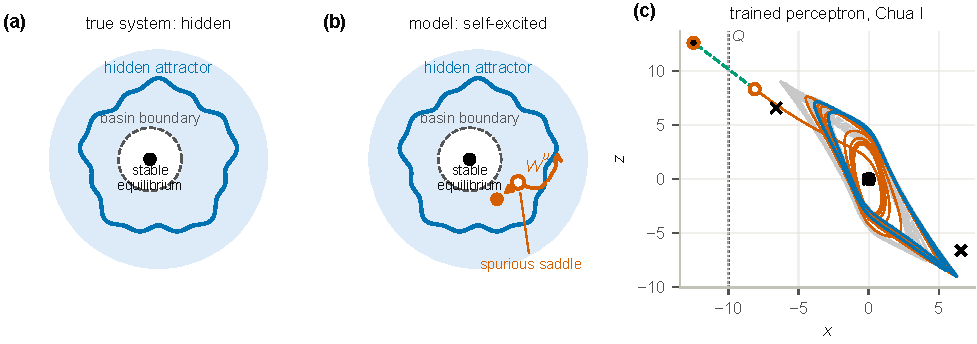
\includegraphics[width=\textwidth]{figures/fig_schematic.pdf}
\caption{How a model loses hiddenness. (a) In the true system the basin of the hidden attractor (shaded) is separated from
the stable equilibrium by a basin boundary, so no trajectory started near the equilibrium reaches the attractor. (b) A
trained model reproduces the attractor but has an additional pair of equilibria; one branch of the unstable manifold $W^u$
of the spurious saddle lands on the attractor, which is therefore excited from the saddle (Proposition~\ref{prop:manifold}).
(c) A real case: a one-layer perceptron with $32$ hidden units trained on Chua's circuit in regime~I (training set HE1),
projected on the $(x,z)$ plane. Gray: the hidden attractor of the true system; blue: the attractor reproduced by the model;
crosses: true equilibria. The model copies the stable origin (black circle) and has two spurious equilibria, a saddle (open
circle) $2.3$ units away from the nearest true saddle-focus, possibly its displaced continuation, and a stable equilibrium
outside the region $Q$ (filled, orange edge; dotted line: the boundary $x=-10$ of $Q$).
One branch of the saddle's unstable manifold (dashed) ends on the spurious stable equilibrium; the other (solid, first $450$
steps) winds onto the reproduced attractor, which is therefore self-excited in the model. Of $20$ such perceptrons trained
with different seeds, $18$ reproduce a hidden attractor, and in $8$ of them a branch of a spurious saddle lands on it.}
\label{fig:schematic}
\end{figure*}

\subsection{Index sum of a bounded map}
\label{sec:degree}

Let $F:\mathbb{R}^N\to\mathbb{R}^N$ be the model map of Sec.~\ref{sec:models}. A fixed point $r^*=F(r^*)$ is
\emph{nondegenerate} if $F$ is differentiable at $r^*$ and $\det\bigl(I-DF(r^*)\bigr)\neq0$; its index is
\begin{equation}
\ind(r^*)=\operatorname{sign}\det\bigl(I-DF(r^*)\bigr).
\label{eq:index}
\end{equation}
For the echo state network with activation $\phi$, $DF(r^*)=\operatorname{diag}\bigl(\phi'(Ar^*+b)\bigr)A$; for hard-tanh activation the diagonal
holds zeros and ones (saturated and linear neurons).

\begin{theorem}[Index sum]
\label{thm:degree}
Let $F$ be continuous with bounded image, $\|F(r)\|_\infty\le R$ for all $r$. Then for every $c>R$ the topological
degree of $\mathrm{id}-F$ on the cube $(-c,c)^N$ with respect to $0$ equals~$1$. If all fixed points of $F$ are
nondegenerate, there are finitely many of them and
\begin{equation}
\sum_{r^*=F(r^*)}\ind(r^*)=1.
\label{eq:indexsum}
\end{equation}
\end{theorem}

This is the Lefschetz--Hopf theorem for a map of a cube into its interior;\cite{GranasDugundji2003Fixed,Deimling1985NFA}
we state it because it applies to every bounded model, whatever the training. For the echo state network $R=1$; for a
perceptron with a bounded output layer $R$ is set by its last weights and bias. The cube is taken strictly larger than the
image because fixed points can lie on its boundary, as they do for hard-tanh networks with saturated neurons. If $F$ only
maps a compact convex set $K$ into its interior, the indices of the fixed points in $K$ sum to $1$, which covers
dissipative models with unbounded output. The index has a direct dynamical reading.\cite{KatokHasselblatt1995Intro}

\begin{lemma}
\label{lem:parity}
For a nondegenerate fixed point, $\ind(r^*)=(-1)^\ell$, where $\ell$ is the number of real eigenvalues of $DF(r^*)$ greater
than~$1$, counted with algebraic multiplicity.
\end{lemma}

\begin{corollary}
\label{cor:counts}
Let all $K$ fixed points of $F$ be nondegenerate and let $U$ be the number of unstable ones. Then
(i) $K$ is odd;
(ii) exactly $(K-1)/2$ fixed points have index $-1$, each of them is unstable, and hence $U\ge(K-1)/2$;
(iii) if a numerically found set $\hat E$ of fixed points has $\sum_{\hat E}\ind\neq1$, then $\hat E$ is incomplete.
\end{corollary}

Item (ii) means that every additional pair of equilibria brings at least one unstable equilibrium, and item (iii) gives a
check of root finding that costs nothing once the Jacobians are known; the converse fails, since a missed pair of indices
$+1$ and $-1$ leaves the sum unchanged. Index sums of this kind constrain the fixed points of threshold-linear networks in
continuous time,\cite{Curto2019TLN,Morrison2024TLN} and degree arguments prove that unstable fixed points exist in
continuous Hopfield networks.\cite{Beise2026UnstableHopfield} For random networks the number of equilibria grows
exponentially with $N$.\cite{WainribTouboul2013,BenArous2021Counting} Theorem~\ref{thm:degree} applies to every closed-loop
echo state network and to every perceptron with a bounded output layer. It does not apply to residual networks,
$F(u)=u+g(u)$ with bounded $g$, nor to next-generation reservoir computers, whose trajectories can escape to infinity.

\subsection{Forced spurious equilibria}
\label{sec:forced}

The true system has its own equilibria, and a good model should have copies of them. Let $\varphi_h$ be the flow map of
the true system over the sampling time $h$ and $x_1,\dots,x_m$ its hyperbolic equilibria in the region $Q$. Let $\ell_j$ be
the number of real positive eigenvalues of the Jacobian $Df(x_j)$ of the vector field, counted with algebraic multiplicity,
and
\begin{equation}
\iota_j=\operatorname{sign}\det\bigl(I-D\varphi_h(x_j)\bigr)=(-1)^{\ell_j},\qquad s=\sum_{j=1}^m\iota_j.
\label{eq:trueindex}
\end{equation}
The second equality is the relation between the index of an equilibrium and that of the translation operator along the
flow:\cite{KrasnoselskiiTranslation1968} since $D\varphi_h(x_j)=\exp\bigl(h\,Df(x_j)\bigr)$, a real eigenvalue $\lambda$
contributes a factor $1-e^{h\lambda}$ of the sign of $-\lambda$, and a complex pair contributes $|1-e^{h\lambda}|^2>0$.

\begin{proposition}[Forced spurious equilibria]
\label{prop:forced}
Let $F$ be continuous with bounded image and all fixed points nondegenerate, and let $r_1,\dots,r_m$ be fixed points with
$\ind_F(r_j)=\iota_j$. Then the remaining fixed points of $F$ have total index $1-s$; if $s\neq1$, there are at least $|1-s|$
of them. The condition $\ind_F(r_j)=\iota_j$ holds if near $r_j$ there is a $C^1$ invariant manifold on which $F$ is
$C^1$-conjugate to $\varphi_h$ near $x_j$ and the block of $DF(r_j)$ transversal to it has no real eigenvalue greater
than~$1$.
\end{proposition}

Since $\iota_j=\operatorname{sign}\det\bigl(-Df(x_j)\bigr)$, $s$ is the degree of $-f$ on any ball that contains exactly
$x_1,\dots,x_m$; if $f$ points into such a ball on its boundary, this degree is $1$ by the Poincar\'e--Hopf theorem. Hence
$s\neq1$ excludes a trapping ball around the equilibria, and a bounded model of such a system must ``close'' the escaping
directions inside its bounded state space. Two cases in this study have $s\neq1$. Chua's circuit in regime~I
(Table~\ref{tab:systems}) has three equilibria with indices $(-1,-1,+1)$, so $s=-1$: a bounded model with copies of all
three needs at least two more, of total index $+2$. The Li--Sprott system used by R\"ohm \textit{et al.}\cite{Rohm2021} has
no equilibria, $s=0$, so every bounded model of it has at least one. The forced equilibria have positive total index and
may well be stable; Proposition~\ref{prop:forced} forces equilibria, not unstable ones. In the other regimes $s=1$ and
spurious equilibria are not forced: their number is set by training. Unbounded models such as residual networks escape
the constraint, whereas architectures that guarantee bounded or dissipative learned
dynamics\cite{Kaptanoglu2021Trapping,Li2022Dissipative,Linot2023Stabilized,Tang2026Dissipative} fall under it.

\subsection{Excitation through unstable manifolds}
\label{sec:manifold}

Hiddenness is decided near the equilibria. Let $\mathcal{A}$ be an attractor with basin
$B=\{x:\operatorname{dist}(F^nx,\mathcal{A})\to0\}$, and let $e\notin\mathcal{A}$ be a hyperbolic fixed point near which $F$
is $C^1$ with $DF(e)$ invertible. Its unstable manifold $W^u(e)$ is the set of points with a backward orbit
$y_0=y$, $F(y_{-n-1})=y_{-n}$, converging to $e$, and the local unstable manifold $W^u_{\mathrm{loc}}(e)$ is the part whose
backward orbit stays in a small neighborhood of $e$. For a tanh echo state network with invertible $A$, $F$ is a
diffeomorphism onto $(-1,1)^N$ and backward orbits are unique.

\begin{proposition}[Excitation criterion]
\label{prop:manifold}
(i) If $W^u(e)\cap B\neq\varnothing$, then $B$ intersects every neighborhood of $e$, i.e., $\mathcal{A}$ is excited
from~$e$. (ii) If $W^u_{\mathrm{loc}}(e)\setminus\{e\}$ does not meet the closure $\bar B$, then some neighborhood of $e$
does not intersect $B$.
\end{proposition}

\begin{corollary}
\label{cor:criterion}
$\mathcal{A}$ is excited from $e$ if and only if $W^u_{\mathrm{loc}}(e)\setminus\{e\}$ meets $\bar B$. In particular, if
$W^u(e)\setminus\{e\}$ does not meet the basin boundary, $\mathcal{A}$ is excited from $e$ if and only if
$W^u(e)\cap B\neq\varnothing$. An exciting equilibrium lies on the basin boundary $\partial B$, since $e\in\bar B$ while its
orbit stays at $e\notin\mathcal{A}$. An asymptotically stable equilibrium never excites an attractor. If all equilibria satisfy the hypotheses above and none lies
in $\mathcal{A}$, the attractor is hidden if and only if no local unstable manifold of an unstable equilibrium
meets~$\bar B$.
\end{corollary}

Part (i) is the reasoning behind the standard procedure of starting trajectories on an unstable manifold to locate
self-excited attractors;\cite{LeonovKuznetsov2013,Dudkowski2016} Corollary~\ref{cor:criterion} states when this test is also
complete. The basin boundary matters: a branch of $W^u(e)$ that crosses a codimension-one basin boundary, for instance the
stable manifold of a boundary saddle, does so robustly, and then both adjacent basins are excited. For hard-tanh networks
with saturated neurons, $DF(e)$ is singular, but $F$ is affine near a fixed point inside a linear region, and
part (ii) holds with the same proof. A practical consequence for high-dimensional models is that, to leading order in the
radius, points of a small ball around $e$ leave along $W^u(e)$ and only their projection on the unstable subspace
$E^u(e)$ matters, so the excitation test can sample directions in $E^u(e)$, of dimension $\dim W^u(e)$, instead of a ball
in $\mathbb{R}^N$ (Sec.~\ref{sec:protocol}).

\subsection{A survival heuristic}
\label{sec:heuristic}

Theorem~\ref{thm:degree} and training together supply unstable equilibria, and by Corollary~\ref{cor:criterion} each of them
destroys hiddenness as soon as its unstable manifold reaches the basin. If each of $U$ equilibria had $\nu$ branches
landing independently in $B$ with probability $p_B$, the probability that the attractor stays hidden would be
\begin{equation}
\Pr(\mathcal{A}\ \text{hidden}\mid U)\approx(1-p_B)^{\nu U},
\label{eq:heuristic}
\end{equation}
with $\nu=2$ for a one-dimensional unstable manifold with a positive eigenvalue ($\nu=1$ if the eigenvalue is below $-1$,
since the map then swaps the two branches) and $p_B$ the fraction of the region occupied by the basin. For
higher-dimensional unstable manifolds $\nu$ is only an effective parameter. Equation~\eqref{eq:heuristic} is a reference curve, not a law:
branches of different equilibria of the same model need not be independent, and where they go depends on the data the
model was trained on. Section~\ref{sec:results} measures the actual dependence on $U$ and compares it with
Eq.~\eqref{eq:heuristic}.

\section{Models, equilibria and labels}
\label{sec:methods}

\subsection{Model ensembles}
\label{sec:ensembles}

\begin{table*}
\caption{Model ensembles. ESN: echo state network; mlp, mlp2: perceptrons with one and two hidden layers; res: residual
network; NG-RC: next-generation reservoir computer; ``all'': the seven regimes of Table~\ref{tab:systems} (pooled statistics use six, with LE1 reported separately). H0: noise-free H1. Training sets
are defined in Sec.~\ref{sec:data}; ``light'' and ``full'' refer to the labeling protocols of Sec.~\ref{sec:protocol}; $W^u$: unstable manifolds traced
(Fig.~\ref{fig:schematic}).}
\label{tab:ensembles}
\begin{ruledtabular}
\begin{tabular}{llllll}
Ensemble & Models & Systems & Data, size & Labels & Sec. \\
\hline
Size sweep & $700$ ESN & all & H1, HE1; $N=50$--$2000$ & light & \ref{sec:esn_law} \\
Full-protocol ensemble & $1138$ ESN & all & H1, HE1, E1, H0; $N=300$--$1000$ & full & \ref{sec:theory_checks}, \ref{sec:esn_law}, \ref{sec:e1} \\
Settings sweep & $200$ ESN & four & HE1; $N=300$ & light & \ref{sec:esn_law} \\
Intervention & $82$ ESN & all & H1 $+$ $0$--$20$ transients; $N=300$, $700$ & light & \ref{sec:data_effects} \\
Benchmark & $754$ hard-tanh ESN & Lorenz & one trajectory; $N=8$--$20$ & exact, full & \ref{sec:theory_checks} \\
No-equilibrium control & $32$ ESN & Li--Sprott & one trajectory; $N=300$ & full & \ref{sec:theory_checks} \\
Model classes & $10\,080$ mlp, mlp2, res & all & H1, HE1, E1; $H=8$--$1024$ & light & \ref{sec:theory_checks}, \ref{sec:classes}, \ref{sec:e1} \\
Example & $20$ mlp & Chua~I & HE1; $H=32$ & $W^u$ & \ref{sec:manifold} \\
Penalty & $840$ mlp2 ($720$ analyzed) & all & H1, HE1; $H=256$, $\lambda_{\mathrm{P}}=0$, $0.1$, $1$ & light & \ref{sec:penalty} \\
E1 controls & $210$ NG-RC, $210$ quadratic & all & subsets of E1 & full, light & \ref{sec:e1} \\
Positive controls & $180$ NG-RC, $360$ quadratic & six & windows of H1, HE1 & full, light & \ref{sec:e1} \\
Saturation & $184$ ESN, rebuilt & six & H1, HE1; $N=100$--$2000$ & light & \ref{sec:theory_checks} \\
Certified enumeration & $960$ mlp, mlp2, res & six & H1, HE1; $H=64$, $256$ & -- & \ref{sec:theory_checks} \\
\end{tabular}
\end{ruledtabular}
\end{table*}


Table~\ref{tab:ensembles} lists the ensembles. Echo state networks are trained by ridge regression of the readout on the
reservoir states driven by the training series,\cite{LukoseviciusJaeger2009Reservoir} with tanh activation, a sparse random
$W$ of spectral radius $\rho$ and the input scale and density given in Appendix~\ref{app:training}. The \emph{size sweep}
varies $N$ from $50$ to $2000$; the \emph{full-protocol ensemble} is labeled with the full protocol below and also supplies
the indices of Sec.~\ref{sec:theory_checks} and the networks trained on E1; the \emph{settings sweep} varies the input scale
and the reservoir density; the \emph{intervention ensemble} keeps each reservoir and refits only the readout on the data
variants of Sec.~\ref{sec:data}. The \emph{benchmark} consists of hard-tanh networks whose fixed points are enumerated
exactly (Sec.~\ref{sec:equilibria}), and the \emph{equilibrium-free control} repeats the setting of R\"ohm
\textit{et al.}\cite{Rohm2021} on the Li--Sprott system, which has no equilibria. The perceptrons and residual networks
are trained by Adam on a one-step loss followed by a four-step rollout loss, for eight hidden widths from $8$ to $1024$ and
$20$ seeds per configuration, on H1, HE1 and E1. Two further ensembles serve as interventions and controls: perceptrons
trained with a penalty on unstable equilibria (Sec.~\ref{sec:penalty}) and models whose function class contains the Euler
step of the true vector field for four of the systems (Sec.~\ref{sec:e1}).

\subsection{Equilibria and their indices}
\label{sec:equilibria}

Equilibria are found by Newton's method from many starting points: uniform points in the range of the map (or in an
enlarged region for unbounded models), states visited during training, and the images of the true equilibria in the
model's state space; for echo state networks deflation\cite{Farrell2015Deflation} pushes Newton away from roots already found.
Each root is refined to machine precision, and its Jacobian gives the index~\eqref{eq:index}, the number of unstable
directions and the number of real eigenvalues greater than $1$. Root finding in high dimension is never guaranteed to be
complete;\cite{SussilloBarak2013,AllgowerGeorg2003Continuation} Corollary~\ref{cor:counts}(iii) provides the check we use,
and Sec.~\ref{sec:theory_checks} adds two more: searches with up to eight times as many starts and, for the
three-dimensional models, a certified enumeration by interval arithmetic.
The survival analyses of echo state networks use only networks whose found equilibria have index sum $1$; for the
perceptrons we report the effect of the same restriction. For unbounded models the
check does not apply, and points to which Newton's method runs off to infinity ($|x|>10^3$ in physical units, where the tanh
units saturate) are discarded.

To test the root finding and the labels against ground truth, we use echo state networks with hard-tanh activation
$\phi(z)=\max(-1,\min(1,z))$, trained by the same ridge regression with $N=8$--$20$. In each of the $3^N$ regions where
every neuron is saturated below, linear or saturated above, the closed-loop map is affine, so all fixed points follow from
small linear systems and a sign check. Exhaustive enumeration over the regions gives the complete set of fixed points,
which piecewise-linear search heuristics do not guarantee.\cite{Eisenmann2023Bifurcations} We keep the $754$ networks whose
enumerated fixed points have residuals below $10^{-9}$.

\subsection{Reproduction and excitation labels}
\label{sec:protocol}

For each hidden attractor of the true system, the model is started from $64$ states on that attractor; an echo state
network is first synchronized on $100$ samples of the true trajectory and then run in closed loop. Trajectories are
iterated for $2\times10^4$ steps; those that do not settle on an equilibrium, do not escape and have the right type (largest
Lyapunov exponent above or below $0.02$ per unit time) define the model attractor, which counts as reproduced if
$\Delta_{\mathrm{att}}<0.2$ and $d_H<0.2$ (Appendix~\ref{app:protocol}).

The excitation test starts trajectories near every unstable equilibrium of the model and records which of them reach the
reproduced attractor, i.e., end close to an orbit on it after the same number of steps (Appendix~\ref{app:protocol}). Following
Corollary~\ref{cor:criterion}, the points are placed along the unstable eigendirections (both signs, real and imaginary parts
of complex eigenvectors) at radii $10^{-6}$, $10^{-4}$ and $10^{-3}$, together with $50$--$64$ random points of the ball of the
same radius; radii are in the normalized coordinates of the model (reservoir coordinates for echo state networks, physical
coordinates divided by their standard deviation otherwise). The smallest radius at which some point reaches the attractor is
the excitation radius $\hat r$. The attractor is labeled \emph{self-excited} if $\hat r\le10^{-6}$, \emph{excited at
radius $\hat r$} if $10^{-6}<\hat r\le10^{-3}$, and \emph{not excited} otherwise. ``Not excited'' marks a candidate hidden
attractor.

The full protocol (Appendix~\ref{app:protocol}) adds a radius grid from $10^{-6}$ to $10^{-1}$ with $200$ points per radius
and up to $20$ unstable directions, and a search for further equilibria near the basin boundary, where any exciting
equilibrium lies (Corollary~\ref{cor:criterion}), with an upper bound on the probability that this search misses an
equilibrium.\cite{Good1953,McAllesterOrtiz2003,BerendKontorovich2013,BenHamou2017MissingMass} An attractor is labeled
\emph{statistically hidden} when it is not excited at any radius and the bound is at most $0.05$; this notion, defined in
Appendix~\ref{app:protocol}, is how hiddenness can be asserted in a high-dimensional model whose equilibria cannot all be
guaranteed. On the $115$ pairs (network, attractor) of the six regimes reproduced in both protocols the labels agree in all
$115$: the $45$ ``not excited'' attractors are statistically hidden, and every statistically hidden attractor is ``not
excited''; in LE1 they agree in $14$ of $16$. The
light protocol is used for the large ensembles.

\subsection{Statistics}
\label{sec:stats}

The unit of analysis is a pair (model, hidden attractor) with the attractor reproduced; Chua's circuit contributes two
hidden attractors per model. Two analyses use one row per model: the full-protocol survival curve (the best-matching hidden
attractor) and the intervention regression (the first hidden attractor). Shares are reported with Wilson $95\%$
intervals. The dependence of survival on $U$ is modeled by logistic regression of ``not excited'' on $\log(1+U)$ with fixed
effects for the regime and, where stated, terms for the training set, the model class, the hidden width and the network
size;\cite{Agresti2013Categorical,McCullaghNelder1989GLM} the contribution of a group of terms is tested by the likelihood
ratio. Pairs from the same training configuration (regime, set, class, width or size, which share data and differ only in
the seed) are not independent, so we also report cluster-robust standard errors with these configurations as clusters. All
counts and fits are produced by the scripts listed in the Data Availability statement.

\section{Results}
\label{sec:results}

\subsection{Checks of the theory and of the numerical pipeline}
\label{sec:theory_checks}

\begin{table*}
\caption{Checks of the theory and of the numerical pipeline. The benchmark consists of hard-tanh networks whose fixed
points are enumerated over all $3^N$ linear regions. Copies are model equilibria within $1\%$ of the half-width of the
region $Q$ (half of its largest edge) from a true equilibrium. For the test in the unstable subspace the reference is the ball test of the full protocol;
the last row counts the $27$ networks in which $32$ random directions missed a self-excited attractor.}
\label{tab:theory}
\begin{ruledtabular}
\begin{tabular}{llll}
Result & Check & Data & Count \\
\hline
Thm.~\ref{thm:degree} & Index sum $1$ & hard-tanh benchmark, exact sets & 754/754 \\
 &  & tanh echo state networks & 997/1004 (7 with even $K$) \\
 &  & one-layer / two-layer perceptrons & 3358/3360 / 3279/3360 \\
 &  & residual networks (theorem not applicable) & 1571/3360 \\
Cor.~\ref{cor:counts} & $U\ge(K-1)/2$ & all models with index sum $1$ & no violation \\
 & Incomplete set flagged & Newton sets of the benchmark & 40/43; 0 false of 711 \\
Prop.~\ref{prop:forced} & Copy has index $\iota_j$ & copies within $1\%$ ($0.1\%$) & 440/474 (334/340) \\
 & Chua~I ($s=-1$): copies of all three & echo state networks; mlp; mlp2; res & 0/96; 0/480; 0/480; 23/480 \\
 & Li--Sprott ($s=0$): $K\ge1$ & echo state networks & 32/32 \\
 & Li--Sprott: reproduced, self-excited & training attractor; unseen torus & 29/29; 0/4 \\
Prop.~\ref{prop:manifold} & Test in $E^u$ & self-excited attractors, benchmark & 884/913 \\
 &  & 32 / 256 / 2048 directions, hard cases & 48 / 60 / 70 of 77 \\
\end{tabular}
\end{ruledtabular}
\end{table*}


\begin{figure}
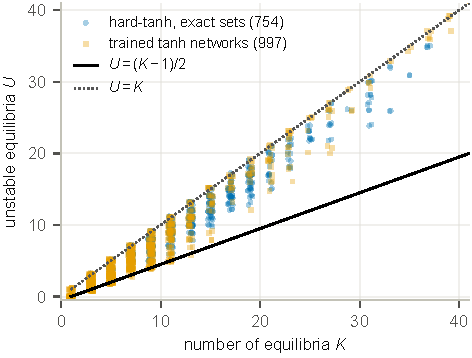
\includegraphics[width=\columnwidth]{figures/fig_theory.pdf}
\caption{Index bookkeeping. Number of unstable equilibria $U$ against the number of equilibria $K$ for the $754$ hard-tanh
benchmark networks with exhaustively enumerated fixed points and the $997$ trained tanh echo state networks of the
full-protocol ensemble (Table~\ref{tab:ensembles}) with index sum $1$; small jitter added. All points lie between the bound
$U=(K-1)/2$ of Corollary~\ref{cor:counts} and $U=K$, and $K$ is always odd.}
\label{fig:theory}
\end{figure}

The theorems need no numerical confirmation; Table~\ref{tab:theory} uses them to validate the numerical pipeline. On the
$754$ hard-tanh benchmark networks ($N=8$--$20$, $K$ between $3$ and $37$), the enumerated indices sum to $1$ in every
network and $K$ is always odd. Among the $1004$ trained tanh echo state networks of the full-protocol ensemble, $997$ have
index sum $1$; the other seven are exactly those with an even number of found equilibria, so their sets are incomplete. The
index sum is $1$ in $3358$ of the $3360$ one-layer and $3279$ of the $3360$ two-layer perceptrons; $76$ of the $81$ two-layer
exceptions have width $512$ or $1024$ and tens to hundreds of equilibria. No network or model with index sum $1$ violates
$U\ge(K-1)/2$ (Fig.~\ref{fig:theory}), and the indices computed from the Jacobians agree with Lemma~\ref{lem:parity} at
all $18\,019$ fixed points of the benchmark and the trained echo state networks, a check of the Jacobians themselves. Residual networks, to which Theorem~\ref{thm:degree} does not apply, have index sum $1$ in
$47\%$ of the cases. Newton's method from the standard starting points missed equilibria in $43$ benchmark networks; in $40$
of them the index sum of the found set differs from $1$, the three sets that pass the check each miss a pair of
equilibria of opposite index, and there are no false alarms.

Two further checks address sets that pass this test and still miss equilibria (supplementary material). For $184$ echo
state networks of the six regimes, rebuilt from the size sweep and from the full-protocol ensemble at $\rho=1.2$, repeating
the search with four ($N\ge700$) or eight ($N\le300$) times as many Newton starts found no further equilibrium in any of the
$136$ networks with $\rho=0.9$, up to $N=2000$ with $33$ unstable equilibria per network on average, and one further unstable
equilibrium in two of the $48$ networks with $\rho=1.2$, neither of which reproduces the hidden attractor; no attractor that
was not excited became excited. In the full-protocol ensemble the $6.8\times10^6$ Newton runs started near the basin
boundaries of candidate hidden attractors found no new equilibrium. For the perceptrons and residual networks we retrained
$960$ models with saved weights, $720$ of them identical to models of Sec.~\ref{sec:classes}, and enumerated their fixed
points by the interval Krawczyk method,\cite{Krawczyk1969Newton,Moore2009Interval} which certifies all fixed points in a box
that contains every fixed point of a bounded model (for residual networks, in $Q$). In every model the certified set equals
the set found by Newton's method.

The forced equilibria of Proposition~\ref{prop:forced} appear where $s\neq1$. An equilibrium of an echo state network that
lies within $1\%$ of the half-width of the region from a true equilibrium (a copy, in what follows) has the index $\iota_j$
of that equilibrium in $440$ of $474$ cases, and in $334$ of the $340$ cases closer than $0.1\%$. The sufficient condition of
Proposition~\ref{prop:forced} cannot be checked directly for trained models; this agreement of indices is the empirical
evidence for its conclusion. The intervention ensemble of Sec.~\ref{sec:data_effects}, whose readout imposes the true
equilibria as exact equilibria of the network, illustrates the bookkeeping: all $66$ networks have index sum $1$ and all
imposed copies, but the copies carry the true indices in only about half of them ($5$ of $16$ in Chua~I), since imposing
the location of an equilibrium does not impose its type (the imposed origin of Chua~I is stable in none of the $16$). Where
they do, the remaining equilibria have total index $1-s$; in Chua~I this forces at least two of them, and these networks
have on average $3.2$, $1.6$ of them stable. For Chua~I ($s=-1$), none of the $96$ echo state
networks and none of the $960$ one- and two-layer perceptrons has copies of all three true equilibria, whereas the
unbounded residual networks have them in $23$ of $480$ cases; the bounded models that copy two of the three (the origin and
one saddle-focus) have spurious equilibria of total index $+1$, on average $2.2$ of them, $1.4$ stable. For the
equilibrium-free Li--Sprott system ($s=0$) every one of the $32$ echo state networks has at least one equilibrium, and all
of these equilibria are unstable. The training attractor, hidden in the true system, is reproduced $29$ times and is
self-excited from these forced equilibria in all $29$; the unseen torus, reproduced in four networks as in the experiment of
R\"ohm \textit{et al.},\cite{Rohm2021} is statistically hidden in all four.

The excitation test in the unstable subspace (Sec.~\ref{sec:manifold}) is efficient but not exhaustive. On the benchmark it
samples the basis directions of $E^u$ and $32$ random directions in it, $37$ points per equilibrium and radius on average
instead of the $1000$ of the reference ball, and finds $884$ of the $913$ self-excited attractors. Once it excites an
attractor that the full protocol had labeled statistically hidden, which shows that a statistically hidden label can be
wrong (one of $46$ on the benchmark). In the $27$ networks with misses, the number of self-excited attractors found grows
from $48$ of $77$ with $32$ directions to $60$ with $256$ and $70$ with $2048$; the seven never found are limit cycles of
networks whose equilibria have unstable subspaces of dimension up to $9$, and whose basins are reached from a tiny
fraction of the directions.

\subsection{Survival law in echo state networks}
\label{sec:esn_law}

\begin{figure*}
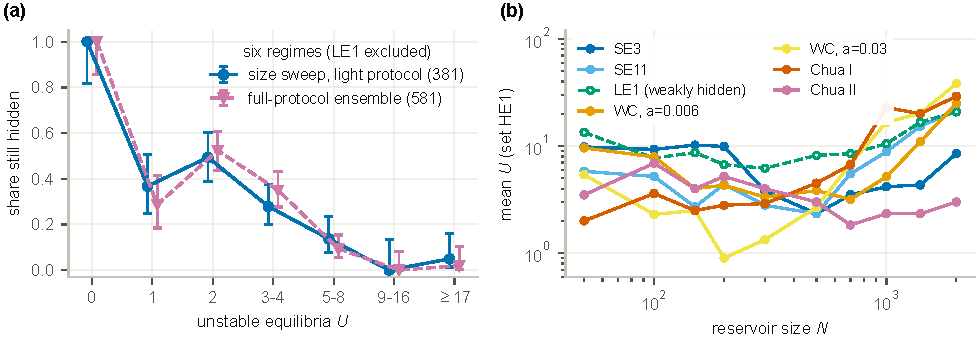
\includegraphics[width=\textwidth]{figures/fig_esn_law.pdf}
\caption{Survival law in echo state networks. (a) Share of reproduced hidden attractors that are not excited from any
unstable equilibrium of the network, against the number $U$ of unstable equilibria, with Wilson $95\%$ intervals; the legend
gives the number of rows; six regimes, LE1 excluded. Solid: size sweep ($620$ networks with $N=50$--$2000$,
Table~\ref{tab:ensembles}), one row per
pair (network, attractor), labeled by the light protocol (balls of radii $10^{-6}$, $10^{-4}$ and $10^{-3}$ around each
unstable equilibrium); dashed: full-protocol ensemble, one row per network, share labeled statistically hidden (not
excited at any radius up to $10^{-1}$, with a bound of at most $0.05$ on the chance that an exciting equilibrium was
missed; Sec.~\ref{sec:protocol}). (b) Mean $U$ against reservoir size for the networks trained on HE1 (the hidden
trajectory plus $20$ transients toward the visible attractor), one line per regime; LE1 dashed.}
\label{fig:esn_law}
\end{figure*}

Figure~\ref{fig:esn_law} shows the survival of reproduced hidden attractors in the size sweep, pooled over the six regimes
whose attractors are hidden in the strict sense: $620$ networks, $776$ pairs (network, hidden attractor), of which $381$ have
the attractor reproduced and index sum $1$. At $U=0$ the attractor is not excited in all $17$ pairs; this point carries no
information beyond the completeness of the equilibrium set, since by Corollary~\ref{cor:criterion} an attractor cannot be
excited without unstable equilibria. One unstable equilibrium brings the share down to $0.37$ $[0.25, 0.51]$, and it
decreases further to $0.14$ at $U=5$--$8$ and $0.05$ at $U\ge17$. The share at $U=2$, $0.49$, exceeds that at $U=1$ because
of the regime mix: $30$ of the $49$ pairs with $U=1$ come from the two Wang--Chen regimes, where none survives, and in no
regime is survival at $U=2$ higher than at $U=1$ (Mantel--Haenszel odds ratio $0.04$ $[0.003, 0.47]$); standardized to
a common regime mix, the shares are $0.60$ $[0.49,0.68]$ at $U=1$ and $0.45$ $[0.38,0.52]$ at $U=2$ (supplementary
material). In a logistic regression with regime fixed effects and terms for the training set and the network size, the
coefficient of $\log(1+U)$ is $-3.08\pm0.40$ (cluster-bootstrap $95\%$ interval $[-4.9,-2.0]$, $380$ networks;
likelihood-ratio $\chi^2=123$), and the decline does not rest on the step from $U=0$: on pairs with $U\ge1$ the coefficient
is $-2.40\pm0.39$. With LE1 added it is $-3.26\pm0.40$. Among links and transformations of $U$, the logit in $\log(1+U)$
has the lowest AIC, and the result is unchanged when the thresholds that define a reproduction are moved from $0.2$ to
$0.1$ or $0.3$ ($-3.25$, $-3.08$). The
network size adds no detectable effect beyond $U$: the coefficient of $\log N$ is $-0.03\pm0.18$ (likelihood-ratio
$p=0.86$), although its $95\%$ interval still allows a change of the log-odds between $-1.7$ and $+1.5$ over the range of
$N$. Size acts mainly through the number of unstable equilibria it produces, which is not monotone in $N$
(Table~\ref{tab:UN}): it grows overall with $N$ for Chua~I, from $2$ at $N=50$ to $29$ at $N=2000$, and has a minimum at
intermediate sizes, between $N=200$ and $700$, for the other regimes trained on HE1.

Two further checks give the same shape. In the full-protocol ensemble, the $581$ networks that reproduce a hidden attractor
(one row per network) keep it statistically hidden in $23$ of $23$ cases at $U=0$, in $0.29$, $0.52$ and $0.35$ of the cases at
$U=1$, $2$ and $3$--$4$ (the same regime mix inverts the first two), in $0.09$ at $U=5$--$8$ and in one of $94$ at $U\ge9$.
Counted by $\Uin$, the unstable equilibria whose physical image $W_{\mathrm{out}}r^*$ lies in $Q$, the decline is monotone:
$0.96$, $0.41$, $0.35$, $0.25$ and $0.03$ at $\Uin=0$, $1$, $2$, $3$--$4$ and $5$--$8$. The coefficient of $\log(1+\Uin)$
is $-3.54\pm0.35$, against $-4.25\pm0.42$ for $\log(1+U)$, and the equilibria outside $Q$ add a smaller effect
($-1.9\pm0.8$); for echo state networks, whose state space is the reservoir, we keep $U$ as the main count. The excitation
came from spurious equilibria alone in $93\%$ of the losses of hiddenness ($383$ of $412$), and from a copy of a true
equilibrium in the rest; the share is $86$--$95\%$ when the distance that defines a copy is halved or doubled. The settings
sweep (SE3, SE11 and Chua~I, $121$ pairs) varies the input scale and the reservoir density and gives a similar coefficient,
$-3.32\pm0.77$; here the settings add an effect beyond $U$ ($\chi^2=17.0$, four degrees of freedom, $p=0.002$), with
coefficients of about $+2$ for the sparser reservoir and for both changed input scales.

The reference curve~\eqref{eq:heuristic} with two branches gives the order of the decay but not its details when $p_B$ is
the basin fraction measured in each network, the share of uniform points of the reservoir cube $[-1,1]^N$ that reach the
reproduced attractor; this is not the $p_B$ of the true system in Table~\ref{tab:systems}. Fitting $\Pr(\text{hidden}\mid U)=q^U$ by maximum likelihood gives $q=0.77$, $0.85$ and
$0.78$ for Chua~I, LE1 and SE3, within $0.03$ of $(1-p_B)^2=0.78$, $0.87$ and $0.81$. For the Wang--Chen system at $a=0.006$,
whose hidden attractor attracts about two thirds of the region, $(1-p_B)^2=0.10$ and the fitted $q$ is close to zero. For SE11
($0.83$ against $0.94$), the cycle of Wang--Chen at $a=0.03$ ($0.18$ against $0.33$) and Chua~II ($0.73$ against $0.99$, $13$
pairs) the observed survival is lower than predicted. Across regimes the heuristic fails as a law: the slopes differ
significantly between regimes (interaction with $\log(1+U)$: likelihood ratio $23$, five degrees of freedom, $p=3\times10^{-4}$),
but by a factor of about two, whereas $\log(1-p_B)$ varies over two orders of magnitude, and a common $\nu$ is rejected.
Survival depends on $U$ in a similar way whether the attractor fills a large or a tiny part of the cube. Equilibria are not
random points of the region, and Sec.~\ref{sec:classes} quantifies how they differ.

\subsection{A similar decline across model classes}
\label{sec:classes}

\begin{table}
\caption{Survival of reproduced hidden attractors: share not excited from any unstable equilibrium, with the number of
pairs (model, hidden attractor) in parentheses, by the number of unstable equilibria: all of them ($U$) for echo state
networks (ESN), those in the region ($\Uin$) for the other classes. ESN: size sweep (Table~\ref{tab:ensembles}); the last
row merges the bins $9$--$16$ and $\ge17$ of Fig.~\ref{fig:esn_law}. Perceptrons (mlp, mlp2) and residual networks (res):
all training sets (H1, E1, HE1; Sec.~\ref{sec:data}). Light protocol (Sec.~\ref{sec:protocol}). Pooled over the six regimes
with strictly hidden attractors; LE1 is reported separately (Sec.~\ref{sec:systems}).}
\label{tab:classes}
\begin{ruledtabular}
\begin{tabular}{lcccc}
$U$ or $\Uin$ & ESN & mlp & mlp2 & res \\
\hline
$0$ & 1.00 (17) & 0.99 (426) & 0.99 (268) & 0.80 (264) \\
$1$ & 0.37 (49) & 0.32 (421) & 0.26 (405) & 0.30 (347) \\
$2$ & 0.49 (79) & 0.18 (154) & 0.28 (130) & 0.28 (286) \\
$3$--$4$ & 0.28 (97) & 0.07 (70) & 0.10 (171) & 0.18 (155) \\
$5$--$8$ & 0.14 (73) & 0.00 (2) & 0.06 (105) & 0.08 (26) \\
$\ge9$ & 0.03 (66) & -- & 0.01 (98) & 0.00 (1) \\
\end{tabular}
\end{ruledtabular}
\end{table}


\begin{figure*}
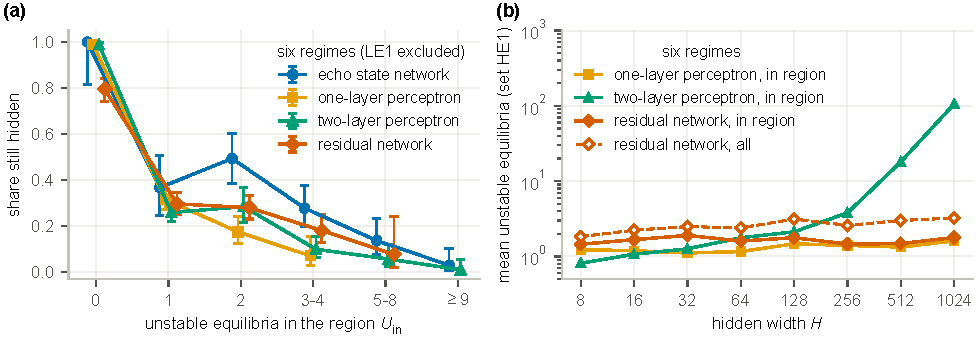
\includegraphics[width=\textwidth]{figures/fig_classes.pdf}
\caption{Survival across model classes. (a) Share of reproduced hidden attractors that stay hidden against the number of
unstable equilibria in the region of the true system, for echo state networks (size sweep, all equilibria counted) and for
one-layer perceptrons, two-layer perceptrons and residual networks (training sets H1, the hidden trajectory; E1, $20$
transients toward the visible attractor; HE1, both); six regimes, LE1 excluded; light protocol, Wilson $95\%$ intervals,
points with fewer than $5$ pairs omitted. (b) Mean number of unstable equilibria against hidden width for models trained on HE1: inside the region
(solid) and, for residual networks, in total (dashed, open symbols).}
\label{fig:classes}
\end{figure*}

The perceptrons and residual networks trained on H1 and HE1 reproduce the hidden attractors in a third to a half of the
cases and lose hiddenness in a similar way (Fig.~\ref{fig:classes}, Table~\ref{tab:classes}). With $\Uin$ counted inside the
region of the true system, the share of attractors that stay hidden falls from $0.99$ at $\Uin=0$ for both perceptrons
($0.80$ for residual networks, whose unstable equilibria outside the region can still excite the attractor) to
$0.26$--$0.32$ at $\Uin=1$ in every class, and to $0.06$ and $0.08$ at $\Uin=5$--$8$ for the two classes that reach these
values. In a logistic regression on the $3329$ reproduced pairs with regime effects, the coefficient of $\log(1+\Uin)$ is
$-3.94\pm0.15$ ($\pm0.24$ with errors clustered by training group of $20$ seeds; cluster-bootstrap interval over the
$3284$ models $[-4.27,-3.67]$; $-3.36\pm0.12$ with LE1). The slope differs between regimes ($p<10^{-6}$), from $-2.7$
in SE11 to $-5.4$ in Wang--Chen at $a=0.006$. Additive class terms are small but not negligible:
$-0.36\pm0.13$ for two-layer perceptrons and $-0.15\pm0.12$ for residual networks ($p=0.002$ for the class). The hidden width
has an effect of $-0.14\pm0.03$ per unit of $\log H$ ($\pm0.07$ cluster-robust). The coefficient of $\log(1+\Uin)$ is
unchanged by terms for the quality of the fit ($\Delta_{\mathrm{att}}$, $d_H$ and training error, $-3.95$), by restricting
to complete equilibrium sets ($-3.94$), by counting attractors excited only at a finite radius as hidden ($-3.88$; there
are $14$ such pairs), by moving the reproduction thresholds to $0.1$ or $0.3$ ($-3.69$, $-4.06$) and by enlarging $Q$ by a
factor of up to two ($-4.06$); halving $Q$ drops equilibria of its outer part and weakens it to $-2.74$. On pairs with
$\Uin\ge1$ it is $-2.74\pm0.22$. The classes are not identical, however: a model with class-specific slopes fits
better (likelihood ratio $82$, two degrees of freedom), with slopes $-5.8$, $-4.1$ and $-2.8$ for one-layer perceptrons,
two-layer perceptrons and residual networks. In a joint fit, echo state networks (slope $-2.2\pm0.3$, counted by $U$)
decline more slowly than both perceptrons and about as fast as residual networks. The class acts mainly, not only,
through $\Uin$.

The classes differ most in how many unstable equilibria they produce. A one-layer perceptron trained on HE1 has on average
$1.1$--$1.6$ unstable equilibria in the region at every width. A two-layer perceptron trained on HE1 has $0.8$ at width $8$,
$3.8$ at width $256$, $18$ at $512$ and $106$ at $1024$; trained on H1, it keeps a reproduced attractor hidden less often
than a one-layer perceptron ($0.28$ against $0.47$). Depth harms hiddenness mainly by creating equilibria. Residual networks have $1.8$ to $3.2$ unstable equilibria on
average, of which $1.5$--$1.9$ lie in the region; counting the others would move them off the common curve. Unstable
equilibria outside the region are not harmless, though: they excite the reproduced attractor in $36\%$ of the cases, which
explains why residual networks keep hiddenness at $\Uin=0$ in only $0.80$ of the cases.

Single equilibria show what the counts hide. An unstable equilibrium inside the region excites the reproduced attractor in
$62\%$ of the cases, against $48\%$ for points of the region at the same distance from the attractor that lie in its basin;
the excess is large in Chua's circuit and SE11 and absent for perceptrons in the Wang--Chen regimes and SE3. Excitation
falls with the distance to the attractor, from $0.88$ within $0.03$ of its diameter to $0.28$ beyond one diameter, and
$77\%$ of the exciting equilibria send part of a small ball elsewhere, as equilibria on a basin boundary
(Corollary~\ref{cor:criterion}) do. Spurious equilibria excite in $63\%$ of the cases, whatever the distance that defines a
copy. Copies of the true saddle-foci of Chua's circuit excite in $68\%$ ($111$ of $164$), although the true saddle-foci do
not: a locally faithful copy does not carry a faithful unstable manifold. Unstable copies of true stable equilibria excite
in $30\%$. Equilibria with one, two and three unstable directions excite in $55\%$, $66\%$ and $66\%$, and unstable foci
excite more often than saddles ($0.67$ against $0.55$). A real eigenvalue below $-1$, which has no counterpart in the flow map of the
true system (its real eigenvalues $e^{h\lambda}$ are positive), is rare: it is the only unstable direction of $51$ of the
$2951$ equilibria with one unstable direction (index $+1$ instead of $-1$), and these excite in $27\%$ of the cases, against
$55\%$ for an eigenvalue above $1$; another $245$ equilibria combine one eigenvalue above $1$ with one below $-1$. If the
equilibria of a model excited the attractor independently with these probabilities, survival would be $0.09$ at
$\Uin=3$--$4$ and $0.03$ at $\Uin=5$--$8$; the observed values are $0.13$ and $0.06$. Excitation is correlated within a
model: in a logistic model of single equilibria with a random effect per model, the latent intra-model correlation is
$0.48$ (median odds ratio $5.2$; likelihood ratio against no random effect $1095$), the population-averaged probability that
an equilibrium inside $Q$ excites the attractor is $0.68$, and this model reproduces the survival curve, which independent
equilibria underpredict. Some models place all their equilibria so that none reaches the basin. In LE1, whose attractor is reached in the true system from a segment of the unstable half-line
of equilibria (Sec.~\ref{sec:systems}), copies of the line excite the reproduced attractor in $16\%$ of the cases and
spurious equilibria in $61\%$, and survival stays at $0.35$--$0.47$ for $\Uin\ge3$: a model that copies the line keeps
part of its weak hiddenness.

\subsection{What the data do}
\label{sec:data_effects}

\begin{figure}
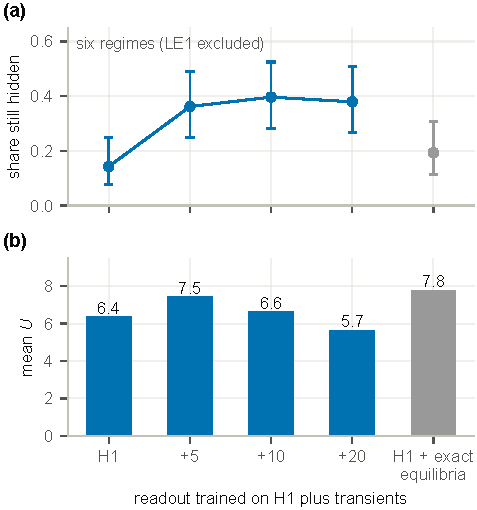
\includegraphics[width=\columnwidth]{figures/fig_intervention.pdf}
\caption{Intervention by data: the reservoirs of $66$ echo state networks (six regimes, LE1 excluded) are kept and only the
readout is refitted on
the hidden trajectory H1 plus $0$, $5$, $10$ or $20$ transients toward the visible equilibrium, or on H1 with the true
equilibria imposed as exact equilibria of the network (gray). (a) Share of reproduced hidden attractors that stay hidden
(first hidden attractor of each network), with Wilson $95\%$ intervals. (b) Mean number of unstable equilibria. Survival
rises with five transients and then levels off; the mean $U$ falls in most regimes and rises in Chua~II; imposing the true
equilibria raises $U$. Light protocol.}
\label{fig:intervention}
\end{figure}

The training set is the main factor beyond $U$. Adding the transients of HE1 to the hidden trajectory raises the odds of
survival at fixed $\Uin$ by a factor of $e^{1.52}\approx4.6$ (coefficient $1.52\pm0.20$ with cluster-robust errors). To
separate this effect from $U$, the intervention ensemble keeps the reservoirs of $66$ echo state networks of the six
regimes ($48$ with $N=300$ and $18$ with $N=700$) and refits only the readout on H1 with $0$, $5$, $10$ or $20$ added
transients (Fig.~\ref{fig:intervention}). The share of reproduced attractors that stay hidden rises from $0.14$
$[0.08, 0.25]$ on H1 to $0.36$, $0.40$ and $0.38$ $[0.27, 0.51]$ with $5$, $10$ and $20$ transients: five transients give
the whole effect. Within a network, going from H1 to E20 lowers $U$ in $38$ of $55$ pairs; hiddenness appears in $17$
pairs, $15$ of them with fewer unstable equilibria and two with the same number, and is lost in three.

In the echo state networks the transients act largely, but not only, through $U$. Within a network, $U$ falls in $33$, $38$
and $38$ of the $55$--$56$ pairs from H1 to E5, E10 and E20, and of the $15$, $18$ and $17$ pairs in which hiddenness appears,
only one has more unstable equilibria. A mediation analysis through $\log(1+U)$ with cluster-bootstrap intervals attributes
$54\%$ $[33,91]$, $61\%$ $[40,100]$ and $77\%$ $[51,129]$ of the effect of E5, E10 and E20 to the change of $U$; the direct
effect is borderline for E5 and E10 and not significant for E20. In a regression on the five described variants with regime
effects and $\log N$, the coefficient of E20 is $1.6\pm0.5$ without and $0.9\pm0.6$ with $\log(1+U)$, whose own coefficient
is $-3.74\pm0.58$. The mean $U$ over all networks rises with five transients ($6.4$ to $7.5$, Fig.~\ref{fig:intervention})
only because it rises by about $29$ in Chua~II, whose networks reproduce nothing on these sets; it falls in Chua~I ($9.9$ to
$3.8$ with E20), SE11 ($6.1$ to $2.6$) and Wang--Chen at $a=0.03$. The transients also shrink the basin of the reproduced
attractor, in all five regimes with reproductions on E20 (Chua~I from $0.22$ to $0.13$ of the reservoir cube). In LE1 the
transients act differently: the share of unstable equilibria that excite the attractor drops from $0.53$ to $0.01$ while
their number grows from $4.8$ to $6.6$, and survival rises from $3$ to $14$ of $16$, far above what
Eq.~\eqref{eq:heuristic} predicts from the changes of $U$ and $p_B$. Constraining the readout so that the true equilibria
become exact equilibria of the network ($W_{\mathrm{out}}r^*=x^*$) raises $U$ in $40$ of the $66$ networks (Chua~I from
$9.9$ to $13.3$) and leaves survival almost unchanged ($0.19$); its positive effect at fixed $U$ ($+1.5\pm0.6$) is offset by
the additional unstable equilibria.

\subsection{Changing U at fixed data}
\label{sec:penalty}

The survival law is observational: $\Uin$ varies with the class, the width and the seed, and something else could vary with
it. The penalty experiment changes $\Uin$ at fixed data, class and seed. Two-layer perceptrons ($H=256$) were trained on H1
and HE1 in the six regimes with a term in the loss that pushes the spectral radius of every equilibrium found in $Q$ below
one, with weight $\lambda_{\mathrm{P}}=0$, $0.1$ or $1$ and the same seeds and minibatches in the three arms ($720$ models,
Appendix~\ref{app:training}). The penalty removes unstable equilibria at an unchanged one-step error: the mean $\Uin$ falls
from $2.70$ to $0.05$ and $0.11$, it decreases in $88\%$ of the paired models and increases in at most $3$ of the $240$, and
the median ratio of the one-step training errors to the unpenalized ones is $0.92$ and $0.99$ (at $\lambda_{\mathrm{P}}=1$ a tenth of the
models fit $2.3$ times worse or more). It removes them indiscriminately, however: in Chua's circuit, whose true unstable
equilibria lie in $Q$, the penalized models have almost none, so they cannot reproduce the true equilibrium structure there. Reproduction drops
from $195$ to $170$ and $162$ of the $320$ pairs (model, hidden attractor), mostly in Chua~II and SE11. Among the reproduced
attractors the share that stays hidden rises from $0.27$ $[0.21,0.34]$ to $0.994$ $[0.97,1.00]$ at both values of $\lambda_{\mathrm{P}}$,
so the number of hidden reproductions triples ($53$, $169$ and $161$). Of the $150$ pairs reproduced both without the
penalty and with $\lambda_{\mathrm{P}}=0.1$, the attractor became hidden in $114$ and lost hiddenness in one (McNemar $p<10^{-32}$).

The penalty acts mainly by moving the models to $\Uin=0$. Of the $332$ penalized reproductions, $325$ have $\Uin=0$, and all
of them keep the attractor hidden. Two-layer perceptrons of the model-class ensemble with the same regime, training set
and $\Uin$ would keep it hidden in $166.5$ of the $170$ penalized reproductions at $\lambda_{\mathrm{P}}=0.1$ and in $157.7$ of
the $162$ at $\lambda_{\mathrm{P}}=1$; $169$ and $161$ are observed (exact $p=0.10$ and $0.05$), so the penalty adds at most
a marginal effect beyond $\Uin$. In a logistic regression on the $527$ reproduced pairs with regime and training-set effects, $\log(1+\Uin)$ and
a step at $\Uin=0$, indicators of $\lambda_{\mathrm{P}}$ add nothing ($\chi^2=0.22$, two degrees of freedom, $p=0.90$), but this test has
little power: the step term is almost separated, and only seven penalized reproductions keep $\Uin\ge1$. The experiment
therefore tests the step from $\Uin\ge1$ to $\Uin=0$, not the curve beyond it. The unstable equilibria that survive the
penalty are nearly neutral (largest spectral radius below $1.05$ in five of the seven), and such equilibria rarely excite
the attractor even without the penalty: at $\lambda_{\mathrm{P}}=0$, models whose unstable equilibria in $Q$ all have a spectral radius below $1.05$ keep it
hidden in $9$ of $11$ cases, against $24$ of $164$ otherwise. Survival depends also on how unstable the equilibria are;
their number is the main variable but not the only one.

The penalty removes saddles by annihilation, not by pushing them out of $Q$: of the $292$ equilibria of index $-1$ inside
$Q$ without the penalty, $285$ and $272$ are gone at $\lambda_{\mathrm{P}}=0.1$ and $1$, the total number of equilibria falls
from $826$ to $260$ and $294$, and the penalized reproductions have no unstable equilibria outside $Q$. Its effect on the
fidelity of the model depends on the data (Sec.~\ref{sec:fidelity}). On HE1 the penalized models keep a stable copy of the
visible equilibrium (all of them, against $78\%$ without the penalty) and are hidden and faithful in $0.64$ of the
reproductions instead of $0.10$; on H1 they hide the attractor without having the visible equilibrium. The share of the true
hidden basin that reaches the reproduced attractor falls, from $0.81$ to $0.73$ at $\lambda_{\mathrm{P}}=0.1$ and from
$0.75$ to $0.54$ at $\lambda_{\mathrm{P}}=1$, and the penalty deletes the copies of the saddle-focus of Chua~II.

In LE1 the penalty makes the model more hidden than the true system: the true attractor is reached from a segment of the
unstable half-line of equilibria (Sec.~\ref{sec:systems}), while the penalized models keep it hidden in all $59$
reproductions, against $17$ of $34$ without the penalty; their remaining unstable equilibria are all nearly neutral. The
penalty is a prior on the equilibria rather than something learned from the data, and it makes the model faithful only
where the true system has no unstable equilibria in $Q$.

\subsection{Hidden is not faithful}
\label{sec:fidelity}

Survival is measured with respect to the model's own equilibria and says nothing about whether the model is right
elsewhere. Three measures that do not depend on these equilibria compare each model with the true system on the uniform
points of $Q$ (supplementary material): the share of points whose outcome in the model corresponds to the true one,
counted over the points that stay bounded in the true system; the share of the true hidden basin that reaches the
reproduced attractor; and whether the model has a stable copy of the visible equilibrium. We call a reproduction faithful
if the model has this copy, at least half of the true hidden basin reaches the reproduced attractor, and the model basin,
restricted to points that stay bounded in the true system, is within a factor of two of the true one.

By these measures survival and fidelity part ways. Models trained on H1, which shows nothing of the visible state, almost
never have a stable copy of the visible equilibrium ($10$ of $800$ one-layer and $3$ of $800$ two-layer perceptrons, $60$ of
$800$ residual networks, $9$ of $278$ echo state networks of the full-protocol ensemble), yet $18$--$34\%$ of their
reproductions stay hidden: there the hidden attractor coexists with spurious stable equilibria, other oscillations or
escape. Of all reproductions by perceptrons and residual networks, $16.5\%$ are hidden and faithful ($27$--$45\%$ on HE1,
under $1\%$ on H1); among echo state networks, $4.6\%$. Within regime, class and training set, the hidden reproductions of
perceptrons and residual networks even have less faithful basins than the excited ones, while for echo state networks they
are slightly more faithful.

The basins of the reproduced attractors are often much too large. In Chua~I the median model basin of one-layer
perceptrons is $0.21$ of $Q$ against $0.020$ per attractor in the true system, but the excess consists of points that escape
to infinity in the true system; on the points that stay bounded, the ratio is close to one. In Chua~II, where nothing
escapes, perceptrons trained on H1 have basins $130$--$160$ times too large, and the transients of HE1 bring them down to a
few times the true size. A model can thus keep a hidden attractor hidden while being far from faithful, and survival is to
be read together with these measures.

\subsection{Training without the hidden attractor}
\label{sec:e1}

\begin{table*}
\caption{Training without the hidden attractor (set E1). Distance: smallest distance from an E1 sample to the hidden
attractor, in units of the attractor's standard deviation per coordinate; coverage: fraction of the attractor within $0.1$
of the E1 data (two values for the two attractors of Chua's circuit). Reproductions are counted over pairs (model, hidden
attractor). Quadratic: sparse quadratic maps fitted by sequential thresholding; NG-RC: next-generation reservoir computer
with the exact quadratic library. LE1, whose attractor is hidden only in a weak sense (Sec.~\ref{sec:systems}), is listed
for completeness.}
\label{tab:e1}
\begin{ruledtabular}
\begin{tabular}{lcccccccc}
Regime & Distance & Coverage & Echo state & mlp & mlp2 & res & Quadratic & NG-RC \\
\hline
SE3 & 0.03 & 0.37 & 1/30 & 5/160 & 0/160 & 3/160 & 0/30 & 23/30 \\
SE11 & 0.11 & 0.00 & 0/19 & 0/160 & 0/160 & 0/160 & 0/30 & 0/30 \\
LE1 & 0.07 & 0.01 & 0/24 & 0/160 & 0/160 & 0/160 & 0/30 & 0/30 \\
WC & 0.55 & 0.00 & 0/18 & 0/160 & 0/160 & 0/160 & 0/30 & 0/30 \\
WC$'$ & 0.40 & 0.00 & 0/18 & 0/160 & 0/160 & 0/160 & 1/30 & 11/30 \\
Chua I & 0.14 / 0.04 & 0.00 / 0.05 & 0/36 & 40/320 & 3/320 & 38/320 & 0/60 & 0/60 \\
Chua II & 1.54 / 1.84 & 0.00 / 0.00 & 0/36 & 0/320 & 1/320 & 0/320 & 0/60 & 0/60 \\
\end{tabular}
\end{ruledtabular}
\end{table*}


Set E1 contains no trajectory on the hidden attractor; it asks whether a model infers the attractor from the transients of
the visible one (Table~\ref{tab:e1}). It does so only where the data nearly show it. In the four regimes where none of
the hidden attractor lies within $0.1$ standard deviations of the E1 data (SE11, both Wang--Chen regimes and Chua~II), one
of the $1920$ perceptrons and residual networks reproduced it. Of the $121$ echo state networks of the six regimes trained
on E1, one reproduced the attractor of SE3, as a self-excited one, and none reproduced any other; in LE1 no model of any
class reproduced it. In SE3 and Chua~I the transients of the visible basin pass along the
attractor itself: in SE3 more than a third of the attractor lies within $0.1$ standard deviations of the E1 data, and in
Chua~I the stable origin attracts so slowly (real part of the eigenvalue $-0.004$) that transients of its basin run beside
the hidden attractor for a long time. There, one-layer perceptrons and residual networks reproduce the attractor in
$2$--$13\%$ of the cases, $69$ of $78$ times the one of the pair closer to the data. This is interpolation rather than
inference of an unseen attractor, and once reproduced, the attractor follows the survival curve: one-layer perceptrons,
mostly with $\Uin\le1$, keep it hidden in $39$ of $45$ cases; residual networks, $37$ of whose $41$ reproductions have
$\Uin=2$--$3$, keep it hidden in one of these $37$.

Two classes whose quadratic library contains the Euler step of the true vector field of SE3, SE11, LE1 and Wang--Chen test
whether the right structure is enough (Appendix~\ref{app:training}); the sampled flow map itself is not quadratic. Sparse
quadratic maps fitted on subsets of E1 reproduced a hidden attractor once in the $180$ maps of the six regimes, the cycle
of Wang--Chen at $a=0.03$, and kept it hidden. In the other maps the points of the true hidden basin go to a
stable equilibrium, to an oscillation that matches no hidden attractor, or to infinity; in SE3, where the Euler step of the
true system lies in the class, $99.8\%$ of them go to the stable equilibrium at the smallest threshold. Trained on the
hidden attractor itself (H1, a random window of three quarters of the trajectory), the same maps reproduce it only in SE3
($6$ of $30$) and for the cycle of Wang--Chen at $a=0.03$ ($20$ of $30$), never in SE11, at $a=0.006$ or in Chua's circuit;
with the transients added (HE1) they reproduce it once in $180$ maps. The class can thus represent the hidden attractor
only in these two regimes, and only there do its failures on E1 bear on inference. Where it reproduces the attractor, it
keeps it hidden in SE3 ($6$ of $6$) and loses it for the cycle ($0$ of $20$, self-excited, mean $\Uin=1.3$).
Next-generation reservoir computers, whose library also contains the Euler step of the four quadratic systems,
reproduced the hidden attractor of SE3 in $23$ of $30$ realizations and the hidden cycle of Wang--Chen at $a=0.03$ in $11$
of $30$, and nothing in the other four regimes or in LE1. Of the $34$ reproductions, $30$ are statistically hidden, $3$ self-excited
and one excited at a finite radius. In SE3 the transients cover a third of the attractor; the cycle of Wang--Chen lies
$0.4$ standard deviations from the nearest E1 sample, so there the model extrapolates. Trained on H1 or HE1, these
computers reproduce the attractor in SE3 and in both Wang--Chen regimes ($74$ of $180$ models) and never in SE11 or Chua's
circuit; their failure on E1 for Wang--Chen at $a=0.006$ is therefore a failure of inference, since the class represents
this attractor ($20$ of $30$ on H1 and HE1). Their survival again follows the unstable equilibria in the region: all $24$
reproductions in SE3 (mean $\Uin\le0.3$) are statistically hidden; for Wang--Chen at $a=0.006$ none of $10$ on H1 (mean
$\Uin=1.7$) and all $10$ on HE1 ($\Uin=0$); for the cycle at $a=0.03$ (mean $\Uin=0.9$--$1.6$) $8$ of $30$. A model with the right structure can thus extrapolate to a hidden attractor, although not reliably;
generic models do not, in agreement with the general impossibility of generalizing across basins without prior
structure.\cite{Goring2024OOD} Inference of unseen attractors from data on one attractor, demonstrated for systems without
equilibria and for visible attractors,\cite{Rohm2021,Norton2025Unseen} was not observed here for generic models (echo state
networks, perceptrons and residual networks, whose function classes do not contain the true vector field) trained on
transients of the visible basin. The training series carry weak dynamical noise ($3\times10^{-4}$--$3\times10^{-3}$ of the
attractor's standard deviation); stronger noise, which lets the data explore the neighborhood of the attractor, was not
tested, and the conclusion is limited to this low-noise regime.

\section{Discussion}
\label{sec:discussion}

Hiddenness is a global property, and training controls a model only near its data. An attractor stays hidden in a model
only if the local unstable manifold of no unstable equilibrium of the model reaches its basin (Corollary~\ref{cor:criterion}).
The model is fitted on the attractor and, at best, on transients toward the visible state; nothing in the loss constrains
where the unstable manifolds of equilibria away from the data go. Topology fixes the bookkeeping of these equilibria: their
number is odd, every additional pair contains an unstable one (Corollary~\ref{cor:counts}), and when the true system has
$s\neq1$, reproducing its equilibria forces additional ones (Proposition~\ref{prop:forced}). How many pairs a model carries is
set by training, and the measured survival curves show how quickly the resulting unstable equilibria cost hiddenness: one in
the region costs about two thirds of the probability of staying hidden, and with nine or more one to three reproduced
attractors in a hundred survive. The decline is similar for echo state networks, one- and two-layer perceptrons and residual networks once
the equilibria are counted where the dynamics lives, which identifies $\Uin$ as the main variable; the class-specific slopes
and the effect of the training set show that it is not the only one.

The two cases with $s\neq1$ show what topology does and does not decide. In Chua's circuit, regime~I,
Proposition~\ref{prop:forced} does not forbid a bounded model to copy all three true equilibria; it requires additional ones
if it does. The bounded models in our ensembles instead miss one of the saddle-foci, while residual networks copy all three
in $23$ of $480$ cases; but the fixed points of a residual network are the zeros of $g\approx h f$, which biases it toward the
equilibria of the flow, so this comparison mixes topology with architecture. Where bounded models have extra equilibria,
these are mostly stable and do not by themselves destroy hiddenness. In the equilibrium-free Li--Sprott system every
bounded model has an equilibrium by Brouwer's theorem, which the true system does not have, and in every one of the $29$
reproductions the training attractor is excited from it. Topology forces the equilibrium, not its excitation; but in all our reproductions the attractor, which has
no equilibrium to be excited from in the true system, is self-excited in the model, an aspect of the reconstruction of
unseen attractors\cite{Rohm2021} that the reconstruction of the attractor itself does not reveal.

Several practical rules follow. After training, the equilibria of a model should be located and, for bounded models, their
index sum checked; Corollary~\ref{cor:counts}(iii) turns this into a free test of the root finding. The number of unstable
equilibria in the region of the true system is a cheap predictor of whether hiddenness survives. With $\Uin=0$ only equilibria outside the
region can excite the attractor, and $94\%$ of the reproductions by perceptrons and residual networks stayed hidden; each
further unstable equilibrium lowers the chance, from $29\%$ at $\Uin=1$ to $13\%$ at $\Uin=3$--$4$ and $1\%$ at nine or more. Survival is not fidelity, however: a model without the visible
equilibrium, or with a basin many times too large, can keep the attractor hidden for the wrong reason, so hiddenness should
be checked together with the basins and the visible state (Sec.~\ref{sec:fidelity}). Selecting among trained
models by $\Uin$ is therefore more useful for this purpose than increasing the size of the network, which acts mainly through
$U$ and can increase it. Removing unstable equilibria during training also keeps the attractor hidden: a penalty on their
spectral radius did so in $0.994$ of the reproductions at an unchanged median one-step error (Sec.~\ref{sec:penalty}). This
optimizes hiddenness rather than fidelity, however: by Corollary~\ref{cor:criterion} a model without unstable equilibria
in the region can only be excited from outside it, and the penalty removes every unstable equilibrium in the region, true
ones included, such as the saddle-foci of Chua's circuit and the unstable half-line of LE1. It is a prior that suits systems
known to have no unstable equilibria there; otherwise the known equilibria must be exempted from it.
Whether a given unstable equilibrium excites the attractor is decided by its unstable manifold, so the excitation test can
sample the unstable subspace instead of a ball in the full state space; for high-dimensional models this saves more than an
order of magnitude of trajectories, at the price of missing basins reached from a tiny fraction of the directions. Including
transients toward the visible attractor in the training set raises survival, in echo state networks for one half to three
quarters through fewer unstable equilibria and in the model classes also at fixed $\Uin$. Finally, a model should not be trusted to reveal a hidden attractor that its data do
not approach, and imposing the true equilibria on the model does not make it more faithful: in our echo state networks it
added unstable equilibria.

These results give a precise form to several observations in the literature. Untrained attractors have been argued to be
intrinsic to learning systems with a bounded state space;\cite{OHagan2025Confabulation} Theorem~\ref{thm:degree} and
Proposition~\ref{prop:forced} make this exact for equilibria and identify when they are forced. Spurious slow modes that
pull closed-loop reservoirs to fixed points\cite{Oishi2026FastSlow} and extra saddles organizing a reservoir's
attractor\cite{Kabayama2025PseudoLorenz} are instances of the spurious equilibria counted here, and the dependence of basin
predictions on warm-up and model structure\cite{ZhangCornelius2023} reflects the same freedom of a model away from its data.
Architectures that guarantee bounded or dissipative learned
dynamics\cite{Kaptanoglu2021Trapping,Linot2023Stabilized,Tang2026Dissipative} remove escape at the cost described by
Proposition~\ref{prop:forced}. The closed-loop echo state network $r\mapsto\tanh(Ar+b)$ is a discrete Lur'e system, the class
in which hidden oscillations were first studied through the Aizerman and Kalman
problems;\cite{LeonovKuznetsov2013,Kuznetsov2019KalmanHidden} trained networks can also have hidden attractors of their own,
which are spurious, as hand-designed Hopfield networks do,\cite{DancaKuznetsov2017Hopfield} and we leave them to a separate
study.

The study has limits. All true systems are low-dimensional, although the models live in up to $2000$ dimensions. The large
ensembles are labeled by the light protocol, whose ``not excited'' marks a candidate; it agreed with the full protocol in all $115$
pairs of the six regimes, and on the benchmark the full protocol itself mislabeled one of $46$ attractors as hidden. A missed exciting
equilibrium would lower $U$ and make the attractor look hidden at the same time; the index-sum check excludes incomplete sets
of bounded models, but a missed pair of opposite indices passes it. Searches with up to eight times the starts found
further equilibria only in two of $184$ echo state networks, both with $\rho=1.2$ and without a reproduced attractor, and
the certified enumeration found none in $960$ three-dimensional models; the largest reservoirs, however, are represented by only eight networks each for $N=1400$
and $2000$. For echo state networks hiddenness is defined in the
reservoir space, the state space of the model as a dynamical system; a user who initializes the network by synchronization
reaches only a neighborhood of the synchronization manifold, the image of the echo state map, which is generically an
embedding of the driving system,\cite{HartHookDawes2020} and we have not measured how far the equilibria of the networks
lie from it. The perceptrons, which act in the physical space, show a similar decline. The survival curve is
an empirical regularity with a heuristic interpretation, not a theorem: equilibria excite the attractor more often than
points at the same distance lie in its basin in some regimes and not in others, their excitations are correlated within a
model, and the slope of the curve differs between regimes by a factor of about two. Residual networks lie outside
Theorem~\ref{thm:degree}, and counting their equilibria in the region of the true system is a choice justified by the data.
The penalty experiment used one architecture, two-layer perceptrons of width $256$, and moved almost all models to
$\Uin=0$: it tests the step from $\Uin\ge1$ to $\Uin=0$ rather than the curve at $\Uin\ge1$, and a variant that spares the
known true equilibria was not run.

\section{Conclusion}
\label{sec:conclusion}

Trained models of dynamics often reproduce hidden attractors but rarely their hiddenness. Degree theory fixes the bookkeeping
of a model's equilibria. When the true equilibria have an index sum different from one, a bounded model must either miss a
true equilibrium or add spurious ones; in an equilibrium-free system every bounded model has an equilibrium, and in all
our reproductions it made the training attractor self-excited. Otherwise
training decides how many unstable equilibria a model has, and an attractor is excited exactly through their unstable
manifolds. Across about $10^4$ models of four classes trained on six regimes, the probability that a reproduced hidden
attractor stays hidden is set mainly by the number of unstable equilibria in the region of the true system, with the class, the
reservoir size and the depth acting mainly through this number. Data from the basin of the visible attractor help; removing unstable equilibria during training keeps the attractor hidden but also removes true
ones; and generic models do not infer a hidden attractor that the data do not touch. Counting and testing the unstable
equilibria of a trained model is therefore a necessary step before its global predictions, and in particular its account of
hidden regimes, can be trusted.

\section*{Supplementary Material}
See the supplementary material for survival curves and slopes per regime, standardized pooled curves with cluster-bootstrap
intervals, a comparison of link functions, the equilibrium-level model with a random effect per model, sensitivity to the
size of $Q$, the reproduction thresholds and the reservoir spectral radius, the fidelity measures and model basins,
the analysis of which equilibria excite the attractor, and the checks of the completeness of the equilibrium sets.

\begin{acknowledgments}
This work received no external funding.

\textbf{Use of generative AI.} The AI assistant Claude (Anthropic) was used to help edit the text of the article and to write the code for the computations. The formulation of the problem, the theory, the choice of the experiments, the analysis of the results, and the conclusions are the author's. All literature references were checked against the Crossref database and arXiv. The author takes full responsibility for the content of the article.
\end{acknowledgments}

\section*{Author Declarations}

\subsection*{Conflict of Interest}
The author has no conflicts to disclose.

\subsection*{Author Contributions}
\textbf{Maksim Elisov:} Conceptualization (lead); Methodology (lead); Software (lead); Validation (lead); Formal analysis (lead); Investigation (lead); Data curation (lead); Visualization (lead); Writing -- original draft (lead); Writing -- review \& editing (lead).

\section*{Data Availability}
The data that support the findings of this study are openly available in Zenodo at
\url{https://doi.org/10.5281/zenodo.24353893}, Ref.~\onlinecite{Elisov2026ESNCode}. The archive contains the code that
generates the test systems and the training sets, trains the models and labels their equilibria and attractors; the results
for every trained model (one JSON record per model); and the scripts that compute every number, table and figure of this
article from these records. Apart from its echo state network modules, the Python library of the archive is that of an
earlier code archive.\cite{Elisov2026Code}

\appendix

\section{Proofs}
\label{app:proofs}

\subsection{Theorem~\ref{thm:degree}, Lemma~\ref{lem:parity} and Corollary~\ref{cor:counts}}

\begin{proof}[Proof of Theorem~\ref{thm:degree}]
Let $K_c=[-c,c]^N$ with $c>R$ and $H(t,r)=r-tF(r)$ for $t\in[0,1]$. If $r\in\partial K_c$, then
$\|r\|_\infty=c>R\ge\|tF(r)\|_\infty$, so $H(t,r)\neq0$ on $\partial K_c$ for all $t$. By homotopy invariance of the
Brouwer degree,\cite{Deimling1985NFA} $\deg(\mathrm{id}-F,\operatorname{int}K_c,0)=\deg(\mathrm{id},\operatorname{int}K_c,0)=1$.
All fixed points lie in $F(\mathbb{R}^N)\subset[-R,R]^N$, a compact subset of $\operatorname{int}K_c$. A nondegenerate fixed
point $r^*$ is isolated: with $J=DF(r^*)$ and $\kappa=\|(I-J)^{-1}\|^{-1}>0$,
$\|r-F(r)\|\ge\kappa\|r-r^*\|-o(\|r-r^*\|)>0$ for $r\neq r^*$ near $r^*$. The fixed-point set is closed and bounded, and its
points are isolated, so it is finite. The degree is the sum of the local indices. The local index at $r^*$ equals
$\operatorname{sign}\det(I-J)$: on a small sphere around $r^*$ the homotopy $(I-J)(r-r^*)+(1-t)\omega(r)$, with
$\omega(r)=r-F(r)-(I-J)(r-r^*)=o(\|r-r^*\|)$, has no zero, and it connects $\mathrm{id}-F$ to the linear map
$I-J$.\cite{Deimling1985NFA,GranasDugundji2003Fixed} This gives Eq.~\eqref{eq:indexsum}.

If instead $F$ maps a compact convex set $K$ with $0\in\operatorname{int}K$ into $\operatorname{int}K$, then for
$r\in\partial K$ the point $tF(r)$ lies on the segment between $0$ and $F(r)$, hence in $\operatorname{int}K$, and again
$H(t,r)\neq0$ on $\partial K$; the indices of the fixed points in $K$ sum to $1$.
\end{proof}

\begin{proof}[Proof of Lemma~\ref{lem:parity}]
$\det(I-J)=\prod_\lambda(1-\lambda)$ over the eigenvalues of $J=DF(r^*)$ with algebraic multiplicity. A complex-conjugate pair
contributes $|1-\lambda|^2>0$, a real $\lambda<1$ a positive factor and a real $\lambda>1$ a negative one; $\lambda=1$ is
excluded by nondegeneracy.
\end{proof}

\begin{proof}[Proof of Corollary~\ref{cor:counts}]
(i) A sum of $K$ numbers $\pm1$ equal to $1$ has $K$ odd. (ii) If $n_\pm$ fixed points have index $\pm1$, then
$n_++n_-=K$ and $n_+-n_-=1$, so $n_-=(K-1)/2$. By Lemma~\ref{lem:parity} a point of index $-1$ has an odd, hence positive,
number of real eigenvalues greater than $1$ and is unstable. (iii) If $\hat E$ contained all fixed points, its index sum
would be $1$ by Eq.~\eqref{eq:indexsum}.
\end{proof}

\subsection{Proposition~\ref{prop:forced} and the remark on $s$}

\begin{proof}[Proof of Proposition~\ref{prop:forced}]
By Theorem~\ref{thm:degree} the indices of all fixed points of $F$ sum to $1$; the copies contribute $s$, so the remaining
fixed points sum to $1-s$, and since each contributes $\pm1$ there are at least $|1-s|$ of them. For the sufficient
condition, let $M_j$ be the $C^1$ invariant manifold through $r_j$ and $\psi_j$ a $C^1$ diffeomorphism conjugating
$F|_{M_j}$ with $\varphi_h$ near $x_j$. Then $T_{r_j}M_j$ is invariant under $DF(r_j)$ and $DF(r_j)|_{T_{r_j}M_j}$ is similar
to $D\varphi_h(x_j)$. In a basis that extends a basis of $T_{r_j}M_j$, $DF(r_j)$ is block upper triangular with diagonal
blocks similar to $D\varphi_h(x_j)$ and the transversal block $T_j$. Hence
$\det\bigl(I-DF(r_j)\bigr)=\det\bigl(I-D\varphi_h(x_j)\bigr)\det(I-T_j)$, and $\det(I-T_j)>0$ by the argument of
Lemma~\ref{lem:parity}, because $T_j$ has no real eigenvalue greater than $1$ (and none equal to $1$, by nondegeneracy of
$r_j$). Thus $\ind_F(r_j)=\iota_j$.
\end{proof}

For the remark after Proposition~\ref{prop:forced}: $\det\bigl(-Df(x_j)\bigr)=\prod(-\lambda)$ has the sign $(-1)^{\ell_j}$, so
$\iota_j$ is the index of the zero $x_j$ of $-f$ and, for a ball $\mathcal{B}$ containing exactly $x_1,\dots,x_m$,
$s=\deg(-f,\mathcal{B},0)$. If $f$ points into $\mathcal{B}$ on $\partial\mathcal{B}$, then $-f$ points outward and is
homotopic to the identity field through fields without zeros on $\partial\mathcal{B}$, so the degree is $1$
(Poincar\'e--Hopf).

\subsection{Proposition~\ref{prop:manifold} and Corollary~\ref{cor:criterion}}

\begin{proof}[Proof of Proposition~\ref{prop:manifold}]
(i) Let $y\in W^u(e)\cap B$ with backward orbit $y_{-n}\to e$. Since $F^n(y_{-n})=y\in B$ and $x\in B$ if and only if
$F(x)\in B$, every $y_{-n}$ lies in $B$, and $B$ meets every neighborhood of $e$.

(ii) By the Hartman--Grobman theorem\cite{Hartman1960Lemma,Grobman1959Homeo,KatokHasselblatt1995Intro} there is a
homeomorphism $\Phi$ near $e$ conjugating $F$ to its linearization $L=\operatorname{diag}(L_s,L_u)$ in coordinates
$x=(x_s,x_u)$, with a norm in which $\|L_s\|\le\lambda<1$ and $\|L_u^{-1}\|\le\mu^{-1}<1$. Choose $\delta>0$ so small that the
ball of radius $\|L_u\|\delta$ lies in the domain of the conjugacy, and let $A_\delta=\{(0,x_u):\delta\le\|x_u\|\le\|L_u\|\delta\}$.
Its image $\Phi^{-1}(A_\delta)$ is a compact subset of $W^u_{\mathrm{loc}}(e)\setminus\{e\}$, disjoint from the closed set
$\bar B$ by assumption, so it has a neighborhood $V$ with $V\cap B=\varnothing$. Take a point $x$ with $\|x\|<\varepsilon$ in the
linear coordinates. If $x_u\neq0$, let $n$ be the first iterate with $\|L_u^nx_u\|\ge\delta$; then $L^nx$ lies within
$\lambda^n\varepsilon$ of $A_\delta$, and $n\ge\log(\delta/\varepsilon)/\log\|L_u\|\to\infty$ as $\varepsilon\to0$. For
$\varepsilon$ small enough $F^n(x)\in V$, so $F^n(x)\notin B$ and hence $x\notin B$. If $x_u=0$, then $F^n(x)\to e\notin\mathcal{A}$,
so again $x\notin B$. Hence the $\varepsilon$-neighborhood of $e$ does not meet $B$.

If $DF(e)$ is singular but $F$ is affine near $e$, $F(x)=e+DF(e)(x-e)$, as for a fixed point of a hard-tanh network inside a
linear region, the same estimate applies directly to $DF(e)$ with the stable part including the zero eigenvalues.
\end{proof}

\begin{proof}[Proof of Corollary~\ref{cor:criterion}]
If $W^u_{\mathrm{loc}}(e)\setminus\{e\}$ does not meet $\bar B$, part (ii) shows that $\mathcal{A}$ is not excited from $e$.
Conversely, let $y\in(W^u_{\mathrm{loc}}(e)\setminus\{e\})\cap\bar B$ with $y_k\in B$, $y_k\to y$. Near the backward orbit of
$y$, which stays near $e$ where $DF$ is invertible, $F$ has a local inverse $F^{-1}_{\mathrm{loc}}$; the points
$F^{-1}_{\mathrm{loc}}(y_k)$ lie in $B$ and converge to $y_{-1}$, so $y_{-1}\in\bar B$, and by induction $y_{-n}\in\bar B$ for all
$n$. Since $y_{-n}\to e$, every neighborhood of $e$ contains points of $\bar B$ and hence of $B$. If $W^u(e)$ does not meet
$\partial B$, then $W^u_{\mathrm{loc}}(e)\setminus\{e\}$ meets $\bar B$ only inside $B$, and by part (i) and the invariance of
$B$ this happens exactly when $W^u(e)\cap B\neq\varnothing$. An asymptotically stable equilibrium $e\notin\mathcal{A}$ attracts a
neighborhood whose points converge to $e$ and therefore are not in~$B$.
\end{proof}

\section{Systems and data}
\label{app:systems}

The test systems are\cite{Molaie2013,JafariSprott2013,WangChen2012,Leonov2011PLA,Stankevich2017}
\begin{align*}
\text{SE3:}\ \ &\dot x=y,\ \ \dot y=z,\ \ \dot z=-3.4x-y-4z+y^2+xy;\\
\text{SE11:}\ \ &\dot x=y,\ \ \dot y=-x+yz,\\
&\dot z=-y-12z+x^2+9xz-1;\\
\text{LE1:}\ \ &\dot x=y,\ \ \dot y=-x+yz,\ \ \dot z=-x-axy-bxz;\\
\text{WC:}\ \ &\dot x=yz+a,\ \ \dot y=x^2-y,\ \ \dot z=1-4x;\\
\text{Chua:}\ \ &\dot x=\alpha\bigl(y-x-f(x)\bigr),\ \ \dot y=x-y+z,\\
&\dot z=-(\beta y+\gamma z),\\
&f(x)=m_1x+\tfrac12(m_0-m_1)\bigl(|x+1|-|x-1|\bigr),
\end{align*}
with $a=15$, $b=1$ for LE1 and $a=0.006$ or $0.03$ for the Wang--Chen system (WC), and
$(\alpha,\beta,\gamma,m_0,m_1)=(8.4562,12.0732,0.0052,-0.1768,-1.1468)$ in regime~I of Chua's circuit and
$(8.4,12,-0.005,-1.2,-0.05)$ in regime~II. The region $Q$ is $[-10,10]^3$, for Chua's circuit
$[-10,10]\times[-10,10]\times[-15,15]$; trajectories leaving a ball of radius $100$ are counted as escaping. Integration uses
the fourth-order Runge--Kutta method with step $0.01$ ($0.0025$ for Chua's circuit, whose piecewise-linear nonlinearity
produces spurious transient chaos at larger steps). The training series carry dynamical noise: after each step
$x\mapsto x+\sqrt{\delta t}\,\sigma_\xi\xi$ with standard normal $\xi$ and $\sigma_\xi$ equal to a fraction $3\times10^{-4}$ (SE3),
$10^{-3}$ (SE11, LE1) or $3\times10^{-3}$ (Wang--Chen, Chua) of the standard deviation of the attractor per coordinate.
Samples are taken at the intervals $\Delta t$ of Table~\ref{tab:systems}. H1 is one trajectory of $10^4$ samples on the
hidden attractor after a washout of $500$; E1 consists of $20$ trajectories of $500$ samples after a washout of $50$,
started at random points of the basin of the visible attractor (for LE1, of the stable part of the line of equilibria);
HE1 is their union. The basin fractions $p_B$ of Table~\ref{tab:systems} come from a census of uniform initial conditions in
$Q$ integrated until they settle.

For the line of equilibria of LE1 we start $24$ trajectories in random directions at distances $10^{-8}$ and $10^{-4}$ from
each of $140$ points $(0,0,z_0)$, $z_0\in[-3,4]$, integrate them with step $0.005$ for $600$ time units and count those that
end on the attractor (within $0.05$ of a reference orbit at $90\%$ of the checks in the last $20$ time units). None of
the trajectories from the stable half-line reaches the attractor. From the unstable half-line, $170$ of the $1920$ trajectories at distance $10^{-8}$
do, all of them from $0.35\le z_0\le2.2$, and the counts at distance $10^{-4}$ are the same within a few percent; the others
escape or return to the stable half-line, except $24$ that have done neither by $T=600$.

The equilibrium-free control is the Li--Sprott system\cite{LiSprott2014} $\dot x=y-x$, $\dot y=-xz+w$, $\dot z=xy-a$,
$\dot w=-by$, which has no equilibria for $a>0$, in the two cases of R\"ohm \textit{et al.}:\cite{Rohm2021} $(a,b)=(2,0.8)$,
where two symmetric limit cycles coexist with a torus, and $(a,b)=(6,0.1)$, where two symmetric chaotic attractors coexist
with a torus. As in that work, the training series is one noisy trajectory ($11\,000$ samples, Euler integration with step
$10^{-3}$ and noise amplitude $0.2$) on one of the symmetric attractors; the networks have $N=300$, $\rho\in\{0.9,1.2\}$, two
ridge parameters and four seeds per case.

\section{Training of the models}
\label{app:training}

\emph{Echo state networks.} The reservoir matrix $W$ has normal entries with density $0.05$, rescaled to spectral radius
$\rho$; $W_{\mathrm{in}}$ is uniform in $[-0.5,0.5]$ (the input scale), $b$ uniform in $[-0.2,0.2]$, and the input is the
state divided by its standard deviation over the training series. Each training series drives the reservoir from $r=0$;
the first states are discarded as washout, and the readout is fitted by ridge regression with parameter $\eta$ on pairs
$(r_k,u_{k+1})$ within each series. The size sweep uses $\rho=0.9$, $\eta\in\{10^{-7},10^{-4}\}$ and several seeds per
$N\in\{50,100,150,200,300,500,700,1000,1400,2000\}$; the full-protocol ensemble uses $\rho\in\{0.6,0.9,1.2\}$, the same two
values of $\eta$ and $N\in\{300,500,700,1000\}$; the settings sweep and the intervention ensemble use $N=300$ and
$\rho=0.9$.

\emph{Next-generation reservoir computers} follow Gauthier \textit{et al.}\cite{Gauthier2021NGRC} with two time delays:
$x_{n+1}=x_n+W\Phi(x_n,x_{n-1})$, where $\Phi$ contains a constant, the six linear terms and all quadratic monomials of the
normalized $(x_n,x_{n-1})$; $W$ is fitted by ridge regression with $\eta\in\{10^{-3},10^{-1},10\}$.

\emph{Sparse quadratic maps} have the form $u_{n+1}=u_n+\Xi^{\top}\theta(u_n)$ on the normalized state, where $\theta$ contains
a constant, the three linear terms and the six quadratic monomials. $\Xi$ is fitted by sequentially thresholded least
squares, a discrete form of SINDy,\cite{Brunton2016SINDy} with thresholds $0.003$, $0.01$ and $0.03$; for SE3, SE11, LE1 and
Wang--Chen the explicit Euler step of the true vector field belongs to this class. In the controls of
Sec.~\ref{sec:e1} each realization of either class is trained on a random subset of $15$ of the $20$ transients of E1,
with $10$ subsets per parameter value. For the positive controls on H1 and HE1 a realization uses a random window of
three quarters of the hidden trajectory, plus, for HE1, a random subset of $15$ transients; there are $10$ realizations
per threshold for the quadratic maps and $5$ per ridge parameter for the reservoir computers, in the six regimes.

\emph{Perceptrons and residual networks} act on the normalized state. For each regime, training set, class and width the
$20$ seeds are trained together on the GPU with Adam, a cosine learning-rate schedule from $3\times10^{-3}$ to $3\times10^{-5}$
and $2\times10^4$ steps; the first $30\%$ of the steps use the one-step error and the rest a rollout error over four steps.
All computations with trained models are in double precision.

\emph{Penalty on unstable equilibria.} In the experiment of Sec.~\ref{sec:penalty} two-hidden-layer perceptrons with $H=256$
are trained as above with one more term in the loss during the rollout phase. Every $50$ steps the equilibria of each model
are located by Newton's method from $768$ fixed starts ($576$ uniform points of $Q$ and $192$ training states). For the
equilibria $u^*$ found inside $Q$ the term $\lambda_{\mathrm{P}}\,\langle\max(0,\rho(DF(u^*))-0.98)^2\rangle$, averaged over the starts,
is added to the loss; $u^*$ is held fixed between searches and the gradient is taken with respect to the weights, ignoring
the implicit dependence of $u^*$ on them. The term pushes the spectral radius of unstable equilibria below one, and it acts
only on equilibria inside $Q$, so an equilibrium can also leave the penalty by moving out of $Q$. An unstable equilibrium of index $+1$ can become stable
this way, while one of index $-1$ can only disappear together with a partner of index $+1$. A tuning run on SE3 (four seeds,
$5\times10^3$ steps, $\lambda_{\mathrm{P}}\in\{0,0.1,1,10\}$) removed all unstable equilibria in $Q$ at $\lambda_{\mathrm{P}}=0.1$ and $1$ without
increasing the median one-step error, while $\lambda_{\mathrm{P}}=10$ increased the error sixtyfold. The experiment uses $\lambda_{\mathrm{P}}\in\{0,0.1,1\}$,
training sets H1 and HE1 and $20$ seeds per regime. The three arms share the seeds and the minibatches, so the comparison
with $\lambda_{\mathrm{P}}=0$ is paired.

\section{Labeling protocol and statistical hiddenness}
\label{app:protocol}

\emph{Reproduction.} For a model attractor with output samples $X$ and a true attractor $Y$,
\begin{equation*}
\Delta_{\mathrm{att}}^2=\sum_{i=1}^3\Bigl[\Bigl(\frac{\langle X_i\rangle-\langle Y_i\rangle}{\langle|Y_i|\rangle}\Bigr)^2
+\Bigl(\frac{\langle|X_i|\rangle-\langle|Y_i|\rangle}{\langle|Y_i|\rangle}\Bigr)^2\Bigr],
\end{equation*}
and $d_H$ is the Hausdorff distance between the sample sets divided by the diameter of $Y$. An attractor is chaotic if its
largest Lyapunov exponent per unit time exceeds $0.02$.

\emph{Light protocol.} Every unstable equilibrium is perturbed along each eigenvector with $|\lambda|>1$ (both signs, real and
imaginary parts) and at $50$ (echo state networks) or $64$ (other classes) random points of the ball, at radii $10^{-6}$,
$10^{-4}$ and $10^{-3}$; the labels are those of Sec.~\ref{sec:protocol}.

\emph{Full protocol.} Following the definition of statistical
hiddenness,\cite{Good1953,McAllesterOrtiz2003,BerendKontorovich2013,BenHamou2017MissingMass} each unstable equilibrium is
probed at radii $10^{-6},10^{-5},\dots,10^{-1}$ with $200$ points per radius in the ball and along up to $20$ unstable
directions. An attractor not reached at any radius up to $10^{-3}$ is a candidate. For a candidate, $10^3$ points within
$10^{-3}$ of its basin boundary are obtained by bisection between basin points and points with other outcomes, and
$2\times10^4$ Newton runs are started near them without deflation. With $f_1$ equilibria found exactly once in $n$ runs, the
probability $M$ that a further run finds a new equilibrium satisfies, with probability at least $1-\alpha$,
\begin{equation*}
M\le\frac{f_1}{n}+\bigl(1+\sqrt2\bigr)\sqrt{\frac{\ln(2/\alpha)}{n}},
\end{equation*}
by the bias of the Good--Turing estimator and the concentration of the missing mass. New equilibria are probed in turn. The
candidate is labeled statistically hidden if the bound at $\alpha=0.025$ is at most $0.05$ and undetermined otherwise. The
bound controls the probability of missing an equilibrium under the search procedure, not under the geometric measure; an
equilibrium with a tiny Newton basin near the basin boundary can remain undetected.

\emph{Excitation test in the unstable subspace} (benchmark networks). For each unstable equilibrium, $32$ (and in the
check of Sec.~\ref{sec:theory_checks} also $256$ and $2048$) random unit directions in $E^u$ are drawn, and points at two
radii along them are integrated; the test is positive if one of them reaches the attractor.

\section{Additional tables}
\label{app:tables}

\begin{table*}
\caption{Mean number of unstable equilibria $U$ of echo state networks in the size sweep, by regime, training set and
reservoir size $N$ (Table~\ref{tab:ensembles}); H1: one trajectory on the hidden attractor, HE1: H1 plus $20$ transients toward the visible attractor.}
\label{tab:UN}
\begin{ruledtabular}
\begin{tabular}{llcccccccccc}
Regime & Set & $50$ & $100$ & $150$ & $200$ & $300$ & $500$ & $700$ & $1000$ & $1400$ & $2000$ \\
\hline
SE3 & H1 & 5.4 & 7.3 & 7.4 & 4.7 & 5.2 & 5.5 & 5.3 & 4.5 & 5.3 & 6.0 \\
SE3 & HE1 & 9.8 & 9.3 & 10.2 & 9.9 & 3.8 & 2.3 & 3.5 & 4.2 & 4.3 & 8.5 \\
SE11 & H1 & 5.7 & 3.5 & 3.9 & 3.7 & 4.8 & 5.3 & 8.0 & 11.8 & 16.8 & 17.2 \\
SE11 & HE1 & 5.8 & 5.2 & 2.7 & 4.4 & 2.8 & 2.3 & 5.5 & 8.8 & 15.3 & 21.2 \\
LE1 & HE1 & 13.4 & 7.7 & 8.7 & 6.7 & 6.2 & 8.2 & 8.5 & 10.5 & 16.7 & 20.8 \\
WC & HE1 & 9.6 & 7.9 & 4.0 & 4.3 & 3.3 & 3.8 & 3.2 & 5.2 & 11.0 & 24.8 \\
WC$'$ & HE1 & 5.4 & 2.3 & 2.5 & 0.9 & 1.3 & 2.7 & 6.8 & 16.7 & 20.2 & 38.2 \\
Chua I & HE1 & 2.0 & 3.6 & 2.5 & 2.8 & 2.9 & 4.5 & 6.7 & 22.8 & 20.0 & 29.2 \\
Chua II & HE1 & 3.5 & 6.9 & 4.0 & 5.2 & 4.0 & 3.0 & 1.8 & 2.3 & 2.3 & 3.0 \\
\end{tabular}
\end{ruledtabular}
\end{table*}


\begin{table*}
\caption{Logistic regressions of ``not excited'' on the number of unstable equilibria and further terms; all fits include
fixed effects for the regime, the intervention fit also $\log N$. Coefficients with standard errors, and cluster-robust
standard errors with the training configuration as cluster where computed. All fits use the regimes with strictly hidden
attractors (six; three in the settings sweep); LE1 is reported separately (Sec.~\ref{sec:systems}).}
\label{tab:regressions}
\begin{ruledtabular}
\begin{tabular}{llll}
 & Term & Coefficient & Cluster-robust s.e. \\
\hline
\multicolumn{4}{l}{\emph{Echo state networks, size sweep} (381 pairs)} \\
 & $\log(1+U)$ & $-3.08\pm0.40$ & $0.71$ \\
 & set H1 (vs HE1) & $-0.73\pm0.39$ & $0.44$ \\
 & $\log N$ & $-0.03\pm0.18$ & $0.22$ \\
 & $\log(1+U)$, pairs with $U\ge1$ & $-2.40\pm0.39$ & $0.63$ \\
\multicolumn{4}{l}{\emph{Echo state networks, settings sweep} (121 pairs; SE3, SE11, Chua I)} \\
 & $\log(1+U)$ & $-3.32\pm0.77$ & -- \\
 & density $0.02$ / $0.2$ (vs $0.05$) & $+1.96\pm0.72$ / $+0.50\pm0.79$ & -- \\
 & input scale $0.2$ / $1$ (vs $0.5$) & $+2.46\pm0.86$ / $+2.22\pm0.83$ & -- \\
\multicolumn{4}{l}{\emph{Perceptrons and residual networks} (3329 pairs)} \\
 & $\log(1+U_{\mathrm{in}})$ & $-3.94\pm0.15$ & $0.24$ \\
 & class mlp2 (vs mlp) & $-0.36\pm0.13$ & $0.25$ \\
 & class res (vs mlp) & $-0.15\pm0.12$ & $0.23$ \\
 & set HE1 (vs H1) & $+1.52\pm0.11$ & $0.20$ \\
 & set E1 (vs H1) & $+1.40\pm0.32$ & $0.45$ \\
 & $\log H$ & $-0.14\pm0.03$ & $0.07$ \\
 & $\log(1+U_{\mathrm{in}})$, pairs with $U_{\mathrm{in}}\ge1$ & $-2.74\pm0.22$ & $0.32$ \\
\multicolumn{4}{l}{\emph{Echo state networks, intervention} (299 rows, first hidden attractor)} \\
 & $\log(1+U)$ & $-3.74\pm0.58$ & -- \\
 & E20 (vs H1), without / with $\log(1+U)$ & $+1.63\pm0.51$ / $+0.91\pm0.62$ & -- \\
 & exact equilibria (vs H1), with $\log(1+U)$ & $+1.47\pm0.63$ & -- \\
\end{tabular}
\end{ruledtabular}
\end{table*}



\clearpage   % place all remaining figures before the reference list
\bibliography{refs}

\end{document}
